%%% The main file. It contains definitions of basic parameters and includes all other parts.

%% Settings for single-side (simplex) printing
% Margins: left 40mm, right 25mm, top and bottom 25mm
% (but beware, LaTeX adds 1in implicitly)
\documentclass[12pt,a4paper]{report}
\setlength\textwidth{145mm}
\setlength\textheight{247mm}
\setlength\oddsidemargin{15mm}
\setlength\evensidemargin{15mm}
\setlength\topmargin{0mm}
\setlength\headsep{0mm}
\setlength\headheight{0mm}
% \openright makes the following text appear on a right-hand page
\let\openright=\clearpage

%% Settings for two-sided (duplex) printing
% \documentclass[12pt,a4paper,twoside,openright]{report}
% \setlength\textwidth{145mm}
% \setlength\textheight{247mm}
% \setlength\oddsidemargin{14.2mm}
% \setlength\evensidemargin{0mm}
% \setlength\topmargin{0mm}
% \setlength\headsep{0mm}
% \setlength\headheight{0mm}
% \let\openright=\cleardoublepage

%% Generate PDF/A-2u
\usepackage[a-2u]{pdfx}

%% Character encoding: usually latin2, cp1250 or utf8:
\usepackage[utf8]{inputenc}

%% Prefer Latin Modern fonts
\usepackage{lmodern}

%% Further useful packages (included in most LaTeX distributions)
\usepackage{amsmath}        % extensions for typesetting of math
\usepackage{amsfonts}       % math fonts
\usepackage{amsthm}         % theorems, definitions, etc.
\usepackage{bbding}         % various symbols (squares, asterisks, scissors, ...)
\usepackage{bm}             % boldface symbols (\bm)
\usepackage{graphicx}       % embedding of pictures
\usepackage{fancyvrb}       % improved verbatim environment
\usepackage{natbib}         % citation style AUTHOR (YEAR), or AUTHOR [NUMBER]
\usepackage[nottoc]{tocbibind} % makes sure that bibliography and the lists
			    % of figures/tables are included in the table
			    % of contents
\usepackage{dcolumn}        % improved alignment of table columns
\usepackage{booktabs}       % improved horizontal lines in tables
\usepackage{paralist}       % improved enumerate and itemize
\usepackage[usenames]{xcolor}  % typesetting in color

% custom packages
\usepackage{pgfplots} % plots

%%% Basic information on the thesis

% Thesis title in English (exactly as in the formal assignment)
\def\ThesisTitle{Suggester implementation for the OpenGrok search engine}

% Author of the thesis
\def\ThesisAuthor{Bc. Adam Hornáček}

% Year when the thesis is submitted
\def\YearSubmitted{2018}

% Name of the department or institute, where the work was officially assigned
% (according to the Organizational Structure of MFF UK in English,
% or a full name of a department outside MFF)
\def\Department{Network and Labs Management Center}

% Is it a department (katedra), or an institute (ústav)?
\def\DeptType{Institute}

% Thesis supervisor: name, surname and titles
\def\Supervisor{Mgr. Vladimír Kotal}

% Supervisor's department (again according to Organizational structure of MFF)
\def\SupervisorsDepartment{Network and Labs Management Center}

% Study programme and specialization
\def\StudyProgramme{Computer Science}
\def\StudyBranch{Software and Data Engineering}

% An optional dedication: you can thank whomever you wish (your supervisor,
% consultant, a person who lent the software, etc.)
\def\Dedication{%
Dedication.
}

% Abstract (recommended length around 80-200 words; this is not a copy of your thesis assignment!)
\def\Abstract{%
Abstract.
}

% 3 to 5 keywords (recommended), each enclosed in curly braces
\def\Keywords{%
{autocomplete} {suggester} {OpenGrok} {index} {Lucene}
}

%% The hyperref package for clickable links in PDF and also for storing
%% metadata to PDF (including the table of contents).
%% Most settings are pre-set by the pdfx package.
\hypersetup{unicode}
\hypersetup{breaklinks=true}

% Definitions of macros (see description inside)
%%% This file contains definitions of various useful macros and environments %%%
%%% Please add more macros here instead of cluttering other files with them. %%%

%%% Minor tweaks of style

% These macros employ a little dirty trick to convince LaTeX to typeset
% chapter headings sanely, without lots of empty space above them.
% Feel free to ignore.
\makeatletter
\def\@makechapterhead#1{
  {\parindent \z@ \raggedright \normalfont
   \Huge\bfseries \thechapter. #1
   \par\nobreak
   \vskip 20\p@
}}
\def\@makeschapterhead#1{
  {\parindent \z@ \raggedright \normalfont
   \Huge\bfseries #1
   \par\nobreak
   \vskip 20\p@
}}
\makeatother

% This macro defines a chapter, which is not numbered, but is included
% in the table of contents.
\def\chapwithtoc#1{
\chapter*{#1}
\addcontentsline{toc}{chapter}{#1}
}

% Draw black "slugs" whenever a line overflows, so that we can spot it easily.
\overfullrule=1mm

%%% Macros for definitions, theorems, claims, examples, ... (requires amsthm package)

\theoremstyle{plain}
\newtheorem{thm}{Theorem}
\newtheorem{lemma}[thm]{Lemma}
\newtheorem{claim}[thm]{Claim}

\theoremstyle{plain}
\newtheorem{defn}{Definition}

\theoremstyle{remark}
\newtheorem*{cor}{Corollary}
\newtheorem*{rem}{Remark}
\newtheorem*{example}{Example}

%%% An environment for proofs

%%% FIXME %%% \newenvironment{proof}{
%%% FIXME %%%   \par\medskip\noindent
%%% FIXME %%%   \textit{Proof}.
%%% FIXME %%% }{
%%% FIXME %%% \newline
%%% FIXME %%% \rightline{$\square$}  % or \SquareCastShadowBottomRight from bbding package
%%% FIXME %%% }

%%% An environment for typesetting of program code and input/output
%%% of programs. (Requires the fancyvrb package -- fancy verbatim.)

\DefineVerbatimEnvironment{code}{Verbatim}{fontsize=\small, frame=single}

%%% The field of all real and natural numbers
\newcommand{\R}{\mathbb{R}}
\newcommand{\N}{\mathbb{N}}

%%% Useful operators for statistics and probability
\DeclareMathOperator{\pr}{\textsf{P}}
\DeclareMathOperator{\E}{\textsf{E}\,}
\DeclareMathOperator{\var}{\textrm{var}}
\DeclareMathOperator{\sd}{\textrm{sd}}

%%% Transposition of a vector/matrix
\newcommand{\T}[1]{#1^\top}

%%% Various math goodies
\newcommand{\goto}{\rightarrow}
\newcommand{\gotop}{\stackrel{P}{\longrightarrow}}
\newcommand{\maon}[1]{o(n^{#1})}
\newcommand{\abs}[1]{\left|{#1}\right|}
\newcommand{\dint}{\int_0^\tau\!\!\int_0^\tau}
\newcommand{\isqr}[1]{\frac{1}{\sqrt{#1}}}

%%% Various table goodies
\newcommand{\pulrad}[1]{\raisebox{1.5ex}[0pt]{#1}}
\newcommand{\mc}[1]{\multicolumn{1}{c}{#1}}


% Title page and various mandatory informational pages
\begin{document}
%%% Title page of the thesis and other mandatory pages

%%% Title page of the thesis

\pagestyle{empty}
\hypersetup{pageanchor=false}
\begin{center}

\centerline{\mbox{
\includegraphics[width=166mm]{../img/logo-en.pdf}}}

\vspace{-8mm}
\vfill

{\bf\Large MASTER THESIS}

\vfill

{\LARGE\ThesisAuthor}

\vspace{15mm}

{\LARGE\bfseries\ThesisTitle}

\vfill

\Department

\vfill

\begin{tabular}{rl}

Supervisor of the master thesis: & \Supervisor \\
\noalign{\vspace{2mm}}
Study programme: & \StudyProgramme \\
\noalign{\vspace{2mm}}
Study branch: & \StudyBranch \\
\end{tabular}

\vfill

% Zde doplňte rok
Prague \YearSubmitted

\end{center}

\newpage

%%% Here should be a bound sheet included -- a signed copy of the "master
%%% thesis assignment". This assignment is NOT a part of the electronic
%%% version of the thesis. DO NOT SCAN.

%%% A page with a solemn declaration to the master thesis

\openright
\hypersetup{pageanchor=true}
\pagestyle{plain}
\pagenumbering{roman}
\vglue 0pt plus 1fill

\noindent
I declare that I carried out this master thesis independently, and only with the cited
sources, literature and other professional sources.

\medskip\noindent
I understand that my work relates to the rights and obligations under the Act No.~121/2000 Sb.,
the Copyright Act, as amended, in particular the fact that the Charles
University has the right to conclude a license agreement on the use of this
work as a school work pursuant to Section 60 subsection 1 of the Copyright Act.

\vspace{10mm}

\hbox{\hbox to 0.5\hsize{%
In ........ date ............	% FIXME!
\hss}\hbox to 0.5\hsize{%
signature of the author
\hss}}

\vspace{20mm}
\newpage

%%% Dedication

\openright

\noindent
\Dedication

\newpage

%%% Mandatory information page of the thesis

\openright

\vbox to 0.5\vsize{
\setlength\parindent{0mm}
\setlength\parskip{5mm}

Title:
\ThesisTitle

Author:
\ThesisAuthor

\DeptType:
\Department

Supervisor:
\Supervisor, \SupervisorsDepartment

Abstract:
\Abstract

Keywords:
\Keywords

\vss}

\newpage

\openright
\pagestyle{plain}
\pagenumbering{arabic}
\setcounter{page}{1}


%%% A page with automatically generated table of contents of the master thesis

\tableofcontents

%%% Each chapter is kept in a separate file
\chapter*{Introduction}
\addcontentsline{toc}{chapter}{Introduction}

Internet has become an unavoidable component of everyday life of billions of people. Among other things, it serves as a
source of knowledge which is available literally at our fingertips. However, it is not possible for a single person to
filter or find relevant information from such a huge dataset. As a result, many search engines emerged which try to
provide this functionality. Sometimes, users do not know for what they are exactly looking or the search engine can
predict for what the user could be looking based on some criteria. These criteria consist mainly of what the user
already typed into the system or the user's search history. Nevertheless; many others may be integrated as well, e.g.
the system can better predict search based on some personal information about the user (age, gender, etc.) or
searches of other users.


Suggester, or autocomplete, functionality tries to achieve this deficiency by giving the user the possibility to choose
from a handful of choices it deemed the most attractive for the user. Therefore, suggester implementations were added to
many search engines (e.g. Google\footnote{\url{http://google.com}}). However, OpenGrok\footnote{\url{http://opengrok.org}}
search engine does not contain any suggester implementation.

\section{Target of the thesis}

The thesis aims to fulfill the following targets:
\begin{itemize}
    \item Integrate suggester functionality into OpenGrok.
    \item Suggestions provided by the suggester should be meaningful and helpful.
    \item The suggester should provide support for rich configuration.
    \item Evaluate the impact of the suggester on the system running the OpenGrok instance.
    \item Evaluate if and how OpenGrok usage changed, that includes:
    \begin{itemize}
        \item Evaluation of the suggester usage.
        \item Evaluation of search results.
    \end{itemize}
\end{itemize}

\section{Structure}

Chapter \ref{chap:opengrok} \textbf{OpenGrok} provides a quick overview of OpenGrok project. What tools it uses and what
makes the OpenGrok project extraordinary.

Chapter \ref{chap:analysis} \textbf{Analysis} discusses problems that arose during the implementation process and how
they were resolved.

Chapter \ref{chap:user} \textbf{User Documentation} contains pictures of the added functionality and explains how it
should be used.

Chapter \ref{chap:program} \textbf{Program Documentation} describes implementation-specific properties of the work.
In other words, how exactly was the new content integrated into the OpenGrok project.

Chapter \ref{chap:impact} \textbf{Impact on the OpenGrok Project} provides detailed description, comparison and
evaluation of the functionality that affected the OpenGrok project.

% Chapter \ref{chap:epilog} % TODO: conclusion has no number so this does not work properly
% \textbf{Conclusion} concludes the work done and lists possible future extensions or enhancementes.

\chapter{OpenGrok}
\label{chap:opengrok}

\section{Overview}
\label{opengrok_overview}
OpenGrok is an open-source search engine written in
Java\footnote{\url{https://en.wikipedia.org/wiki/Java\_(programming\_language)}}
freely available at \url{https://github.com/oracle/opengrok} under CDDL
license\footnote{\url{https://en.wikipedia.org/wiki/Common\_Development\_and\_Distribution\_License}}.
However, OpenGrok is different to most of the search engines which purpose is to traverse web and find the most relevant
webpages. OpenGrok provides searching across codebases. For instance, if you would like to know which files are using
\textit{mmap} function in \textit{Linux kernel}\footnote{\url{https://en.wikipedia.org/wiki/Linux\_kernel}} then
OpenGrok is the tool for that purpose. It understands a variety of
programming languages, e.g. Java, C, C\#, JavaScript and many others. The code analysis is done by
Ctags\footnote{\url{https://en.wikipedia.org/wiki/Ctags}}.
The other most notable features of OpenGrok are:
\begin{itemize}
    \item Support for multiple projects.
    \item Support for authentization and authorization (\cite{OpengrokAuthLayer}). For instance, by using LDAP
        \footnote{\url{https://en.wikipedia.org/wiki/Lightweight_Directory_Access_Protocol}}.
    \item Support for multiple version control systems\footnote{\url{https://en.wikipedia.org/wiki/Version\_control}},
        e.g. git, mercurial, etc.
        \begin{itemize}
            \item Support for searching in repository history.
            \item Possibility to annotate a file.
            \item Possibility to see history for a specific file.
        \end{itemize}
    \item Support for cross-referencing.
    \item Support for navigation in source files. For instance, by providing list of methods.
    \item Syntax highlighting of source files.
\end{itemize}

\section{Modules}
\label{opengrok_modules}

OpenGrok is split into multiple modules:
\begin{itemize}
    \item jrcs – Java library which provides support for RCS\footnote{\url{https://en.wikipedia.org/wiki/Revision\_Control\_System}}
    version control system.
    \item Indexer – described in \ref{indexer}.
    \item Web – described in \ref{opengrok-web}.
    \item plugins – contains authorization plugins.
    \item distribution – does not contain any code and serves for combining all of the above into one distribution unit.
\end{itemize}

Visualization of these modules and how they are dependent on each other can be seen on figure \ref{opengrok_modules_img}.
\begin{figure}[htbp]
\centering
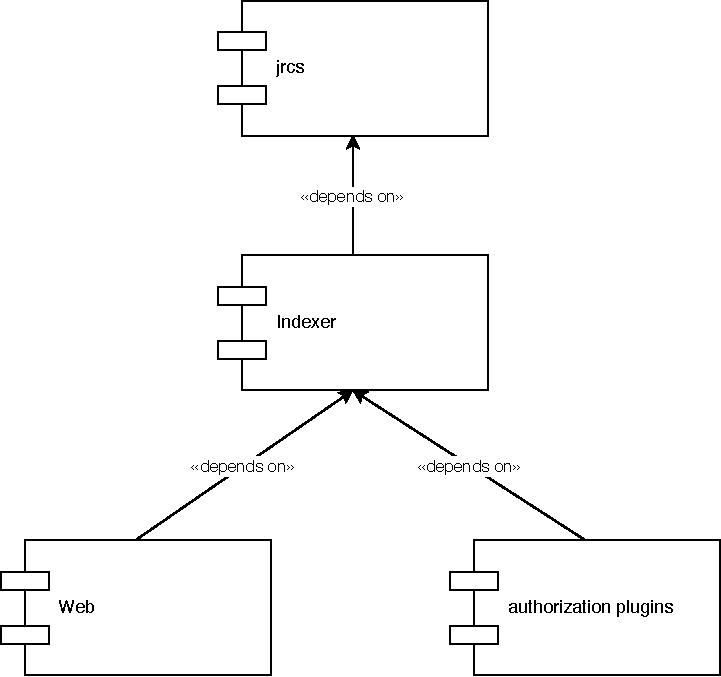
\includegraphics[width=100mm]{../img/opengrok_modules.pdf}
\caption{OpenGrok modules}
\label{opengrok_modules_img}
\end{figure}

Multiple modules support in one project is achieved by Maven\footnote{\url{https://maven.apache.org}} build tool.
There is one main \textit{pom.xml} in the root of the project which aggregates all the modules.

\subsection{Indexer}
\label{indexer}

Indexer is a submodule which main purpose is for each project to:
\begin{itemize}
    \item Generate main lookup index. Detailed description in \ref{indexer:index}.
    \item Generate history index for repositories. Detailed description in \ref{indexer:history}.
    \item Generate xref. Detailed description in \ref{indexer:xref}.
\end{itemize}

\subsubsection{Index}
\label{indexer:index}

OpenGrok heavily relies on Apache Lucene\footnote{\url{https://lucene.apache.org}} \citep{lucene_in_action}, a search engine library
written in Java. Every source file is considered to be a \textit{document}. Every \textit{document} has multiple
\textit{field}s which contain text data. This text data is then tokenized by specific rules (e.g. remove stop words,
stemming, etc.) into tokens. In the Lucene context \textit{term} is a pair of \textit{field} and \textit{token}.
Lucene uses \textit{reverse document index}\footnote{\url{https://en.wikipedia.org/wiki/Inverted_index}},
i.e. for each term a collection of document identifiers is stored in which this term occurrs.
This form of data representation is very efficient for document lookup.

\paragraph{Tokenization}
% TODO: should be here?

\paragraph{Lucene internals}
% TODO: rewrite this? http://lucene.apache.org/core/7_3_1/core/org/apache/lucene/codecs/lucene50/Lucene50PostingsFormat.html

\subsubsection{History}
\label{indexer:history}

OpenGrok uses history index for quick access to history information of every file in a project. OpenGrok first discovers
what kind of version control system the project is using and then executes appropriate commands to retrieve the project's
history (e.g. some form of \textit{git log}). Since executing these commands is not very efficient (new process has to
be created), OpenGrok does this at the indexing phase to provide better performance later. Serialized form of Java object
is stored for each source file of the project to represent its history.

\subsubsection{Xref}
\label{indexer:xref}

Main purpose of the OpenGrok is to find relevant documents based on the search query. After the successful search, the most
obvious route of action is to look at the found documents. However, analyzing the document once again, performing syntax
highlighting and other operations can be very time consuming. Therefore, \textit{xref} directory contains pre-generated
HTML\footnote{\url{https://en.wikipedia.org/wiki/HTML}} versions of every source file which already contain the
aforementioned information.

\subsection{Web}
\label{opengrok-web}

The previous section \ref{indexer:index} describes how the data are processed to create index. However, these data need
to be presented to the end user. Web submodule serves exactly this purpose. It is distributed as a
WAR\footnote{\url{https://en.wikipedia.org/wiki/WAR\_(file\_format)}} which can be used by many
servlet containers\footnote{\url{https://en.wikipedia.org/wiki/Web\_container}}. OpenGrok correctly runs in
Apache Tomcat\footnote{\url{http://tomcat.apache.org}}; nevertheless, there is no Tomcat vendor lock-in; therefore,
other servlet containers should work properly as well.

\subsubsection{Configuration}
\label{opengrok_configuration}

Since OpenGrok has two modules (Indexer and Web) which can be run separately, it needs a way how to pass relevant
information between those. However, it might be possible that Indexer finished its work after a long period of time
(in some cases it might take days) and the Web module is not reachable. Therefore, to not lose all of the information
needed by Web module the Indexer stores it as a read-only configuration. It is stored as an
XML\footnote{\url{https://en.wikipedia.org/wiki/XML}} encoded class which needs to be read by Web on its startup.
If Web module does not find the configuration on the expected place (can be configured in \textit{web.xml}) then an
error is shown on the main page and the usage is not possible. Of course, there are ways how to change the configuration
of the running OpenGrok application via the REST API \footnote{\url{https://en.wikipedia.org/wiki/Representational\_state\_transfer}}
described in the \ref{opengrok_rest}.

\subsubsection{REST API}
\label{opengrok_rest}

Opengrok provides REST API support. This is a relatively new feature. Before that, OpenGrok has known a concept of
\textit{Messages} – custom serialization of Java objects passed to Web application via custom port.
So far most of the REST API calls can be only made from the machine on which the OpenGrok runs.
This is mainly because these REST API calls are meant as a means of communication between Indexer and Web application
or for administrators maintaining the OpenGrok instance. More information can be found at
\url{https://github.com/oracle/opengrok/wiki/Web-services}.

\section{Usage}
\label{opengrok_usage}
The main purpose of the OpenGrok project is to provide ability to search codebases of software projects. This is done
mainly through its web interface. The main OpenGrok page can be seen on the figure \ref{opengrok_main}.

\begin{figure}[htbp]
    \centering
    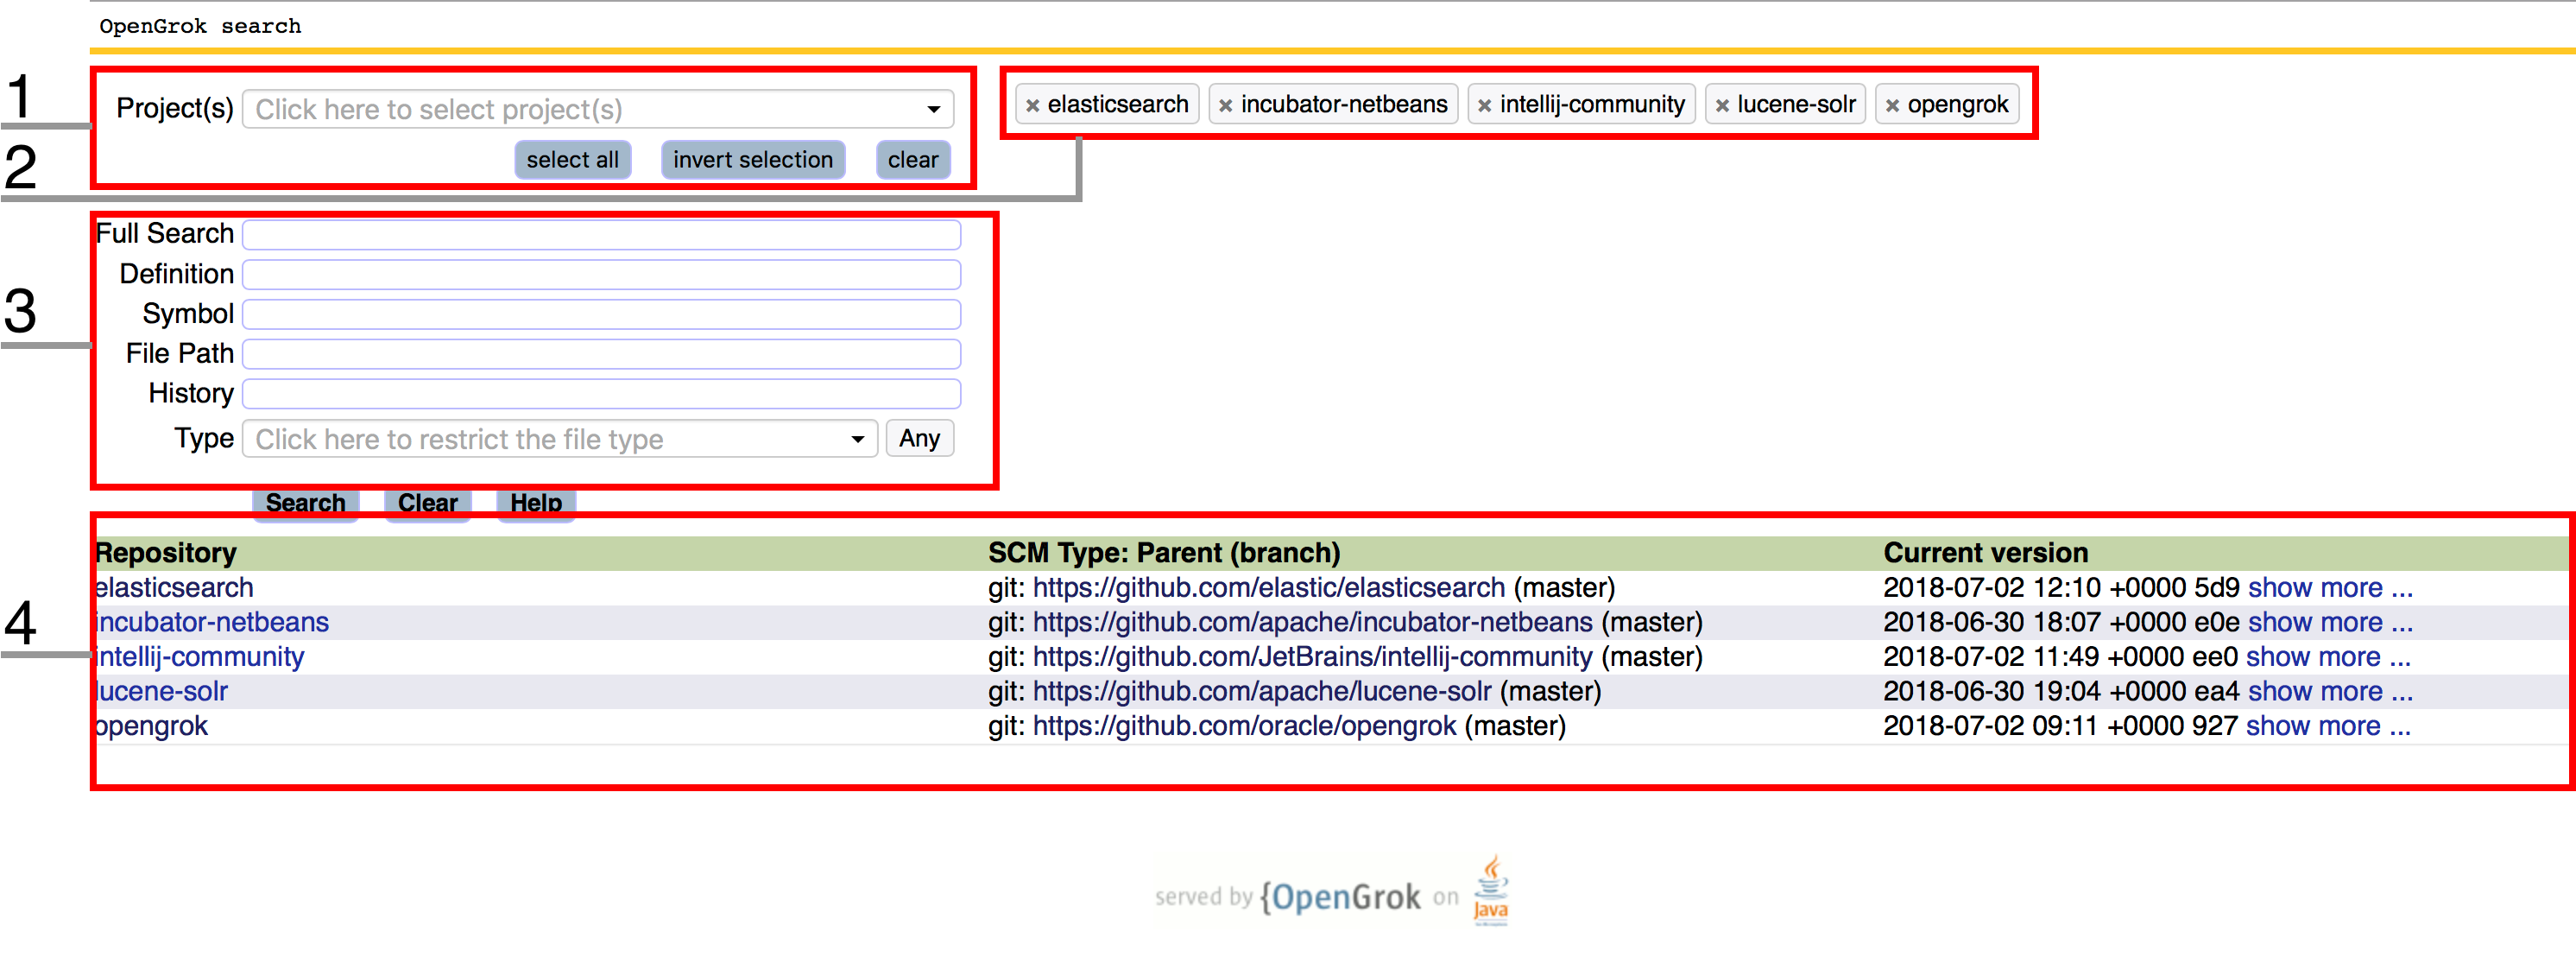
\includegraphics[width=145mm]{../img/opengrok_main.png}
    \caption{Main OpenGrok page}
    \label{opengrok_main}
\end{figure}

The numbers in the figure \ref{opengrok_main} signify:
\begin{enumerate}
    \item Field where projects can be selected.
    \item Selected projects.
    \item Search fields.
       \begin{itemize}
        \item \textbf{Full search} – specifies the text the document should contain. Represents \textit{full} field in
        underlying Lucene implementation.
        \item \textbf{Definition} – specifies the definition of which symbol the document should contain.
        Represents \textit{defs} field in underlying Lucene implementation.
        \item \textbf{Symbol} – specifies the symbol the document should contain.
        Represents \textit{refs} field in underlying Lucene implementation.
        \item \textbf{File Path} – specifies the path the document should have.
        Represents \textit{path} field in underlying Lucene implementation.
        \item \textbf{History} – specifies the history the document should have.
        Represents \textit{hist} field in underlying Lucene implementation.
        \item \textbf{Type} – restricts the search for documents of the type.
        Represents \textit{type} field in underlying Lucene implementation.
       \end{itemize}
    \item Repository list.
\end{enumerate}

It is possible to add values to multiple search fields to make the search more specific. Into the search fields can be
typed any query written in Lucene syntax.

More detailed information with examples can be found on \textit{/help.jsp} web page of the running OpenGrok Web application instance.

\subsection{Navigating results}

\subsection{Traversing source code}

\section{Similar Tools}
It is hard to compare because all of these tools are complex and each of them provides unique feel and solution to problems.
Therefore, the list will only mention if those tools contain suggester functionality. Still, this might not be the best
indicator because they might provide different solutions, e.g. instant search which might make the suggester a redundant asset.
List of similar tools:
\begin{itemize}
    \item \textbf{SourceGraph} \url{https://about.sourcegraph.com} – SourceGraph does support instant search feature.
    While writing some text to the search field it immediately displays the files in which the text was found. The figure
    \ref{sourcegraph} shows how this feature looks like.

    \begin{figure}[htbp]
        \centering
        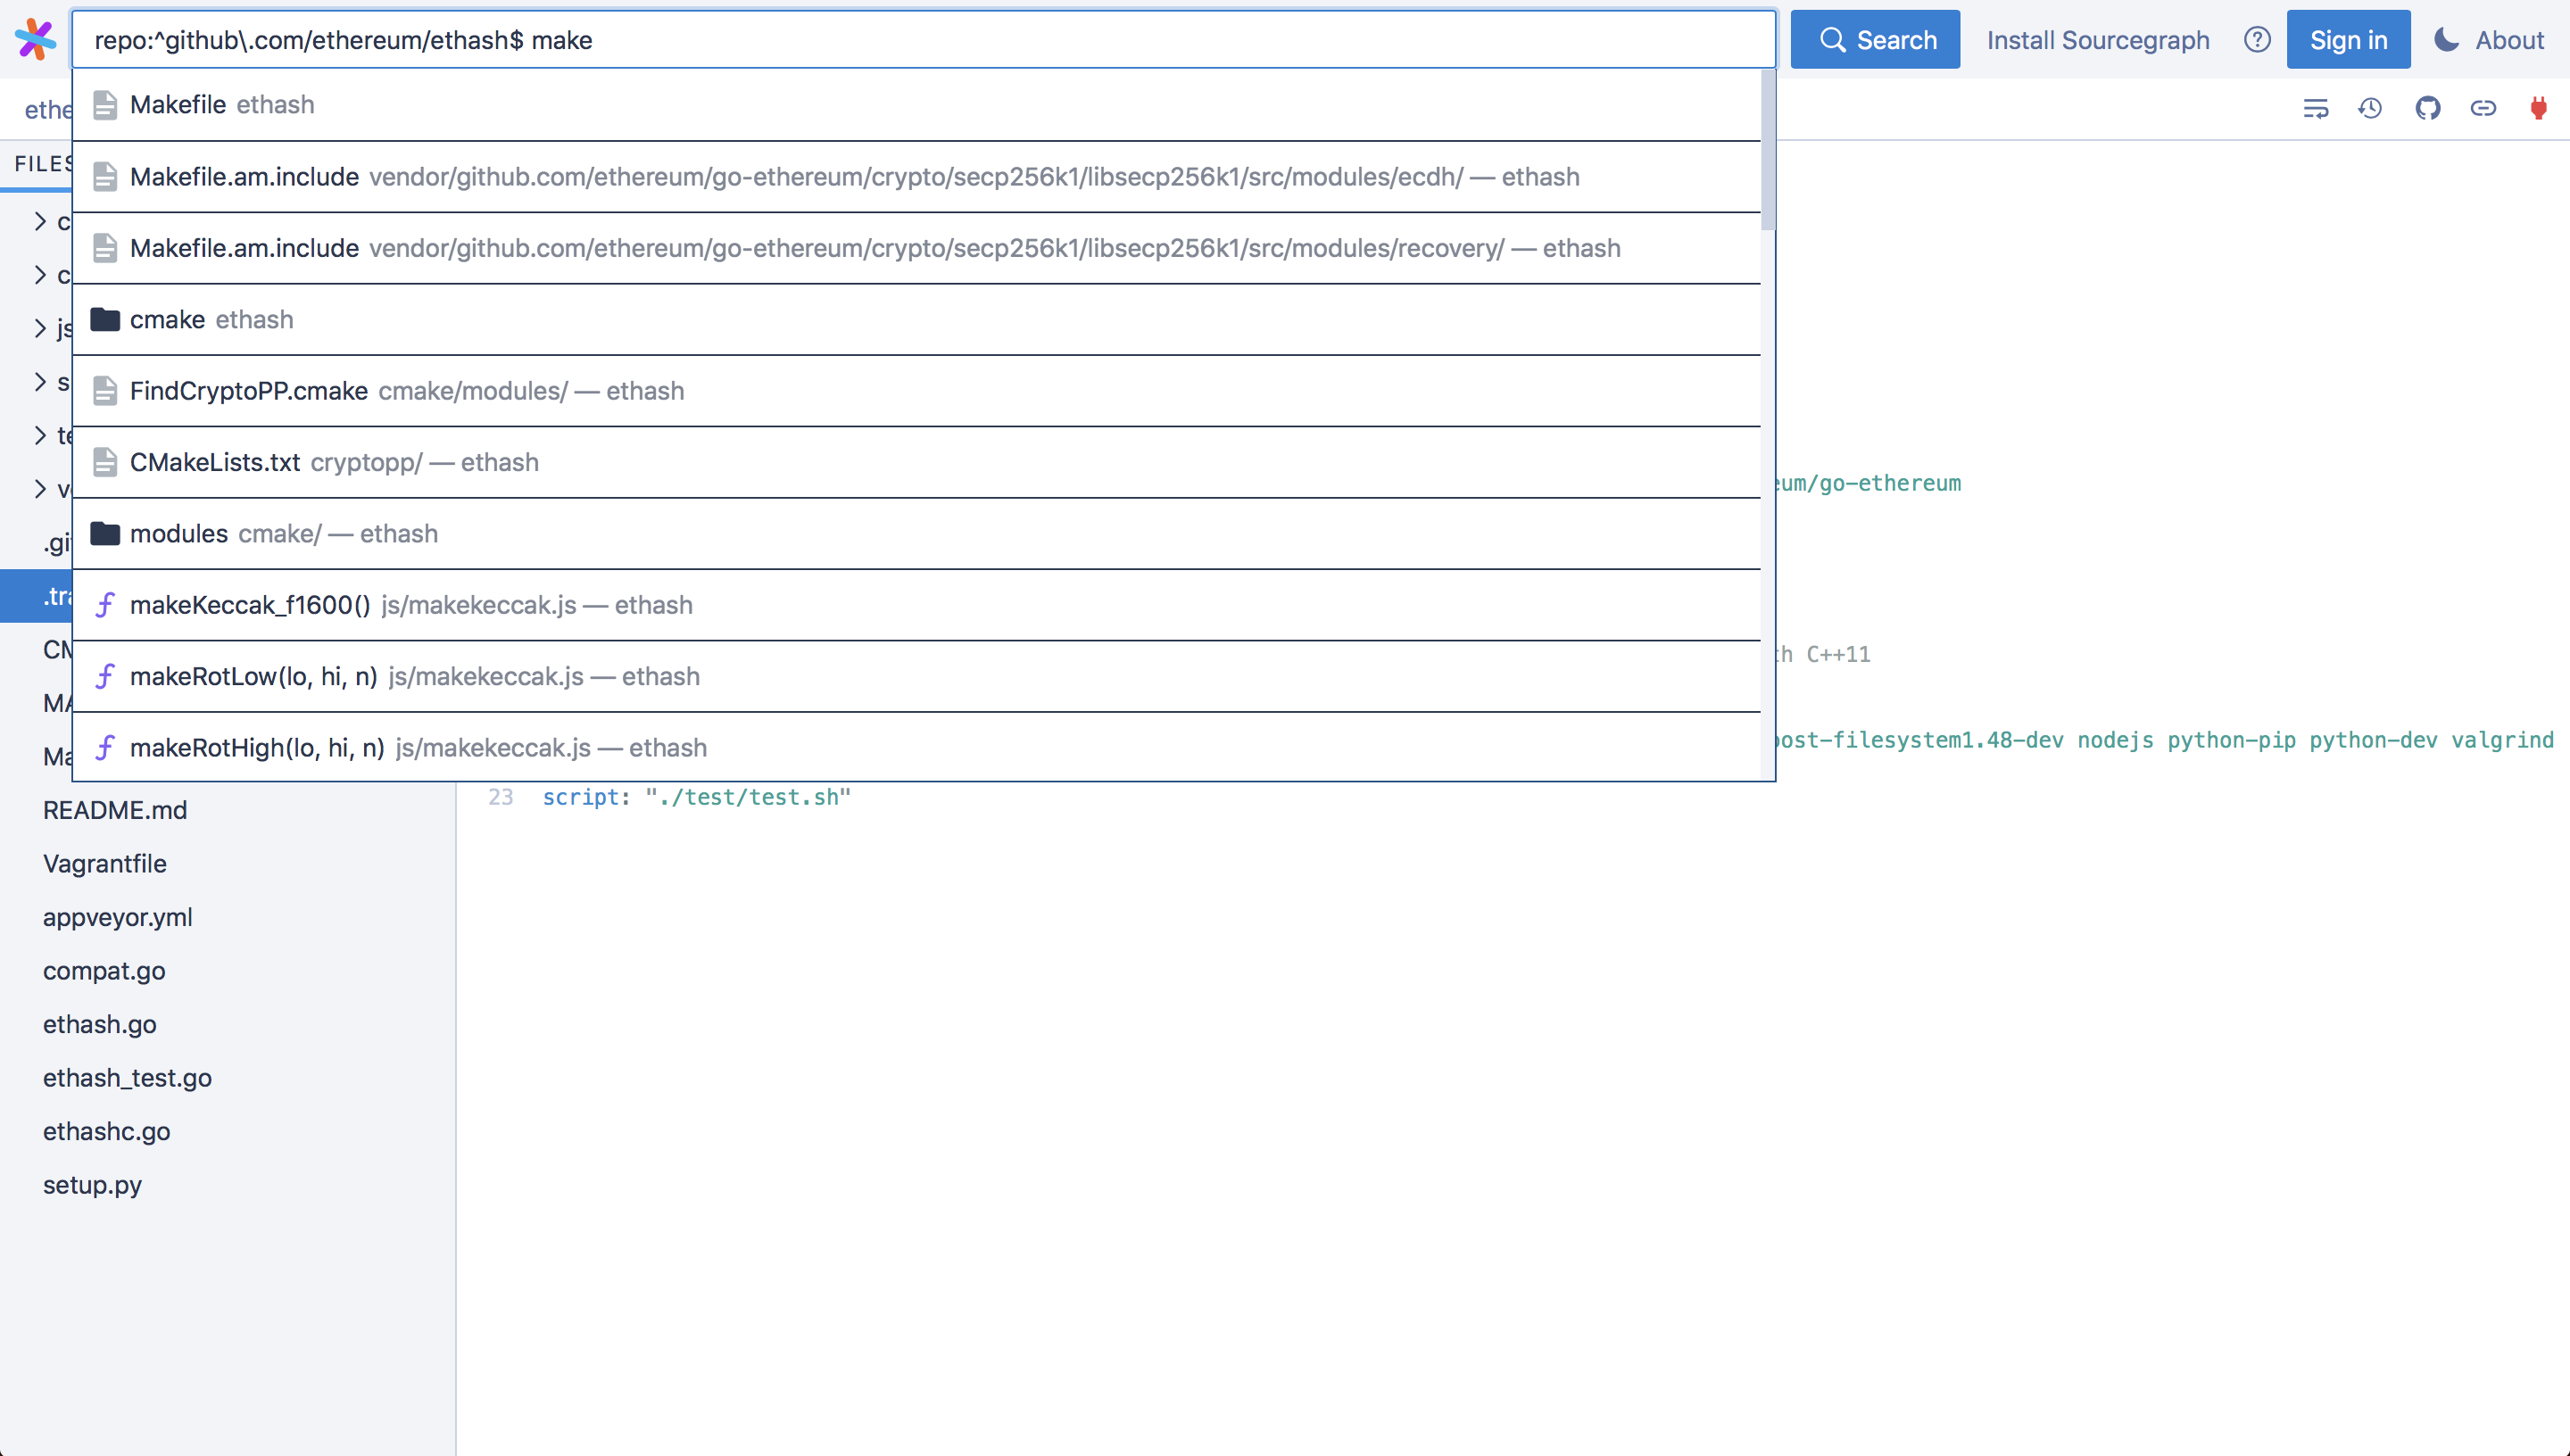
\includegraphics[width=145mm]{../img/sourcegraph.png}
        \caption{SourceGraph instant search feature}
        \label{sourcegraph}
    \end{figure}

    \item \textbf{searchcode} \url{https://searchcode.com/} – it seems that searchcode does not support neither
    autocomplete or instant search feature.

    \item \textbf{livegrep} \url{https://livegrep.com/} – supports instant search. Immediately shows files and their contents
    where the text was found. The look of this application can be seen on figure \ref{livegrep}.

    \begin{figure}[htbp]
        \centering
        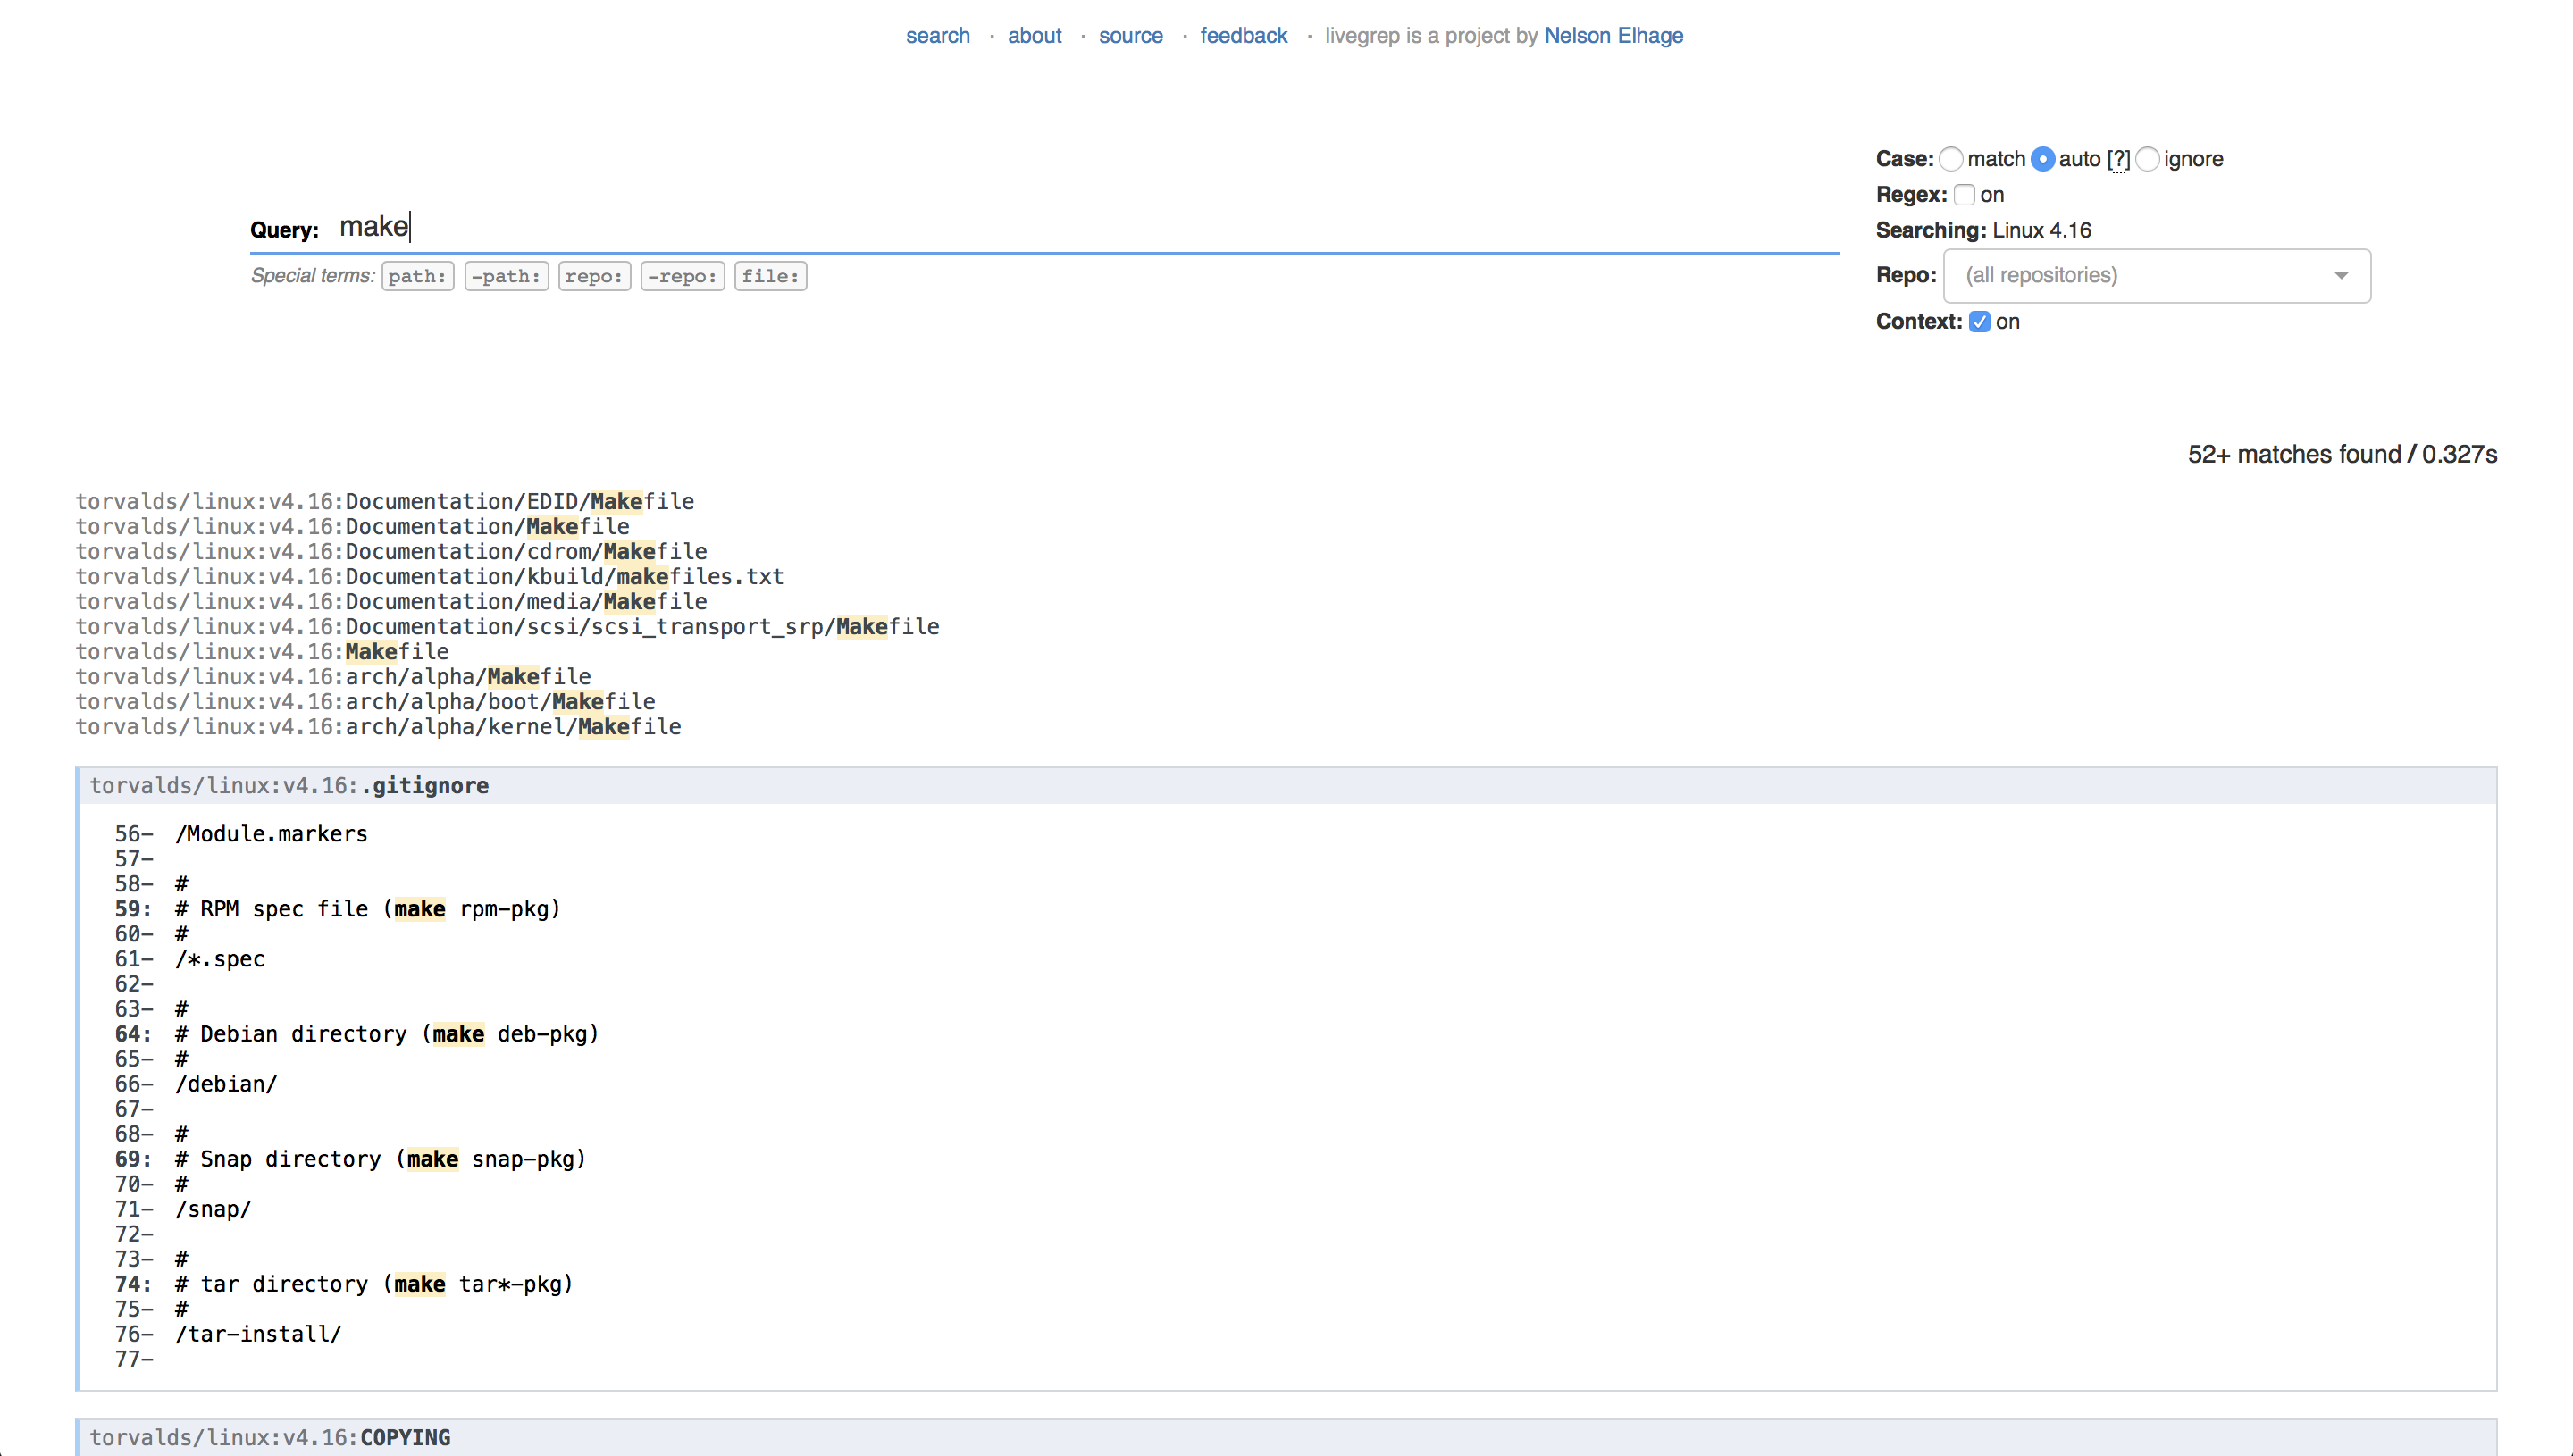
\includegraphics[width=145mm]{../img/livegrep.png}
        \caption{livegrep instant search feature}
        \label{livegrep}
    \end{figure}

\end{itemize}

\chapter{Analysis}
\label{chap:analysis}

This chapter is dedicated to the problems that arose during the work on the project and explains the major decisions
that were made. Chapter is divided into the following sections:
\begin{itemize}
    \item \ref{general_architecture} \textbf{General Architecture} – explains the chosen suggester architecture and
    how it could be combined into the overall OpenGrok architecture.
    \item \ref{opengrok_modifications} \textbf{Opengrok Modifications} – describes the major modifications that had
    to be made in OpenGrok code to enable suggester functionality.
    \item \ref{suggester_module} \textbf{Suggester} – provides detailed explanation how the suggester functionality
    was implemented.
\end{itemize}

\section{General Architecture}
\label{general_architecture}
One of the most important aspects of software products is their architecture. If architecture does not count with some
quality attributes then they are very hard to implement in the underlying code. When designing high level architecture,
there were multiple solutions from which to choose:
\begin{itemize}
    \item \textbf{Implement suggester in the Web module} – probably the easiest solution. There would be no inter-tier
    boundaries; therefore, no need to define public API
    \footnote{\url{https://en.wikipedia.org/wiki/Application\_programming\_interface}}. Also, there would be no need
    to add any other configurations to build scripts. However, this seems like a step towards a monolithic application
    \footnote{\url{https://en.wikipedia.org/wiki/Monolithic\_application}} which proved to be harder to maintain in the
    long run.
    \item \textbf{Implement suggester as a separate module} – suggester could be implemented as an additional module to
    already modular architecture described in \ref{opengrok_modules}. This new module could be a dependency of the Web
    module which would need to be modified to parse and process the data that are passed in. These data then could be
    passed to the new module via its public API. The result would look like shown on a figure \ref{opengrok_modules_changed_img}.
    \begin{figure}[htbp]
    \centering
    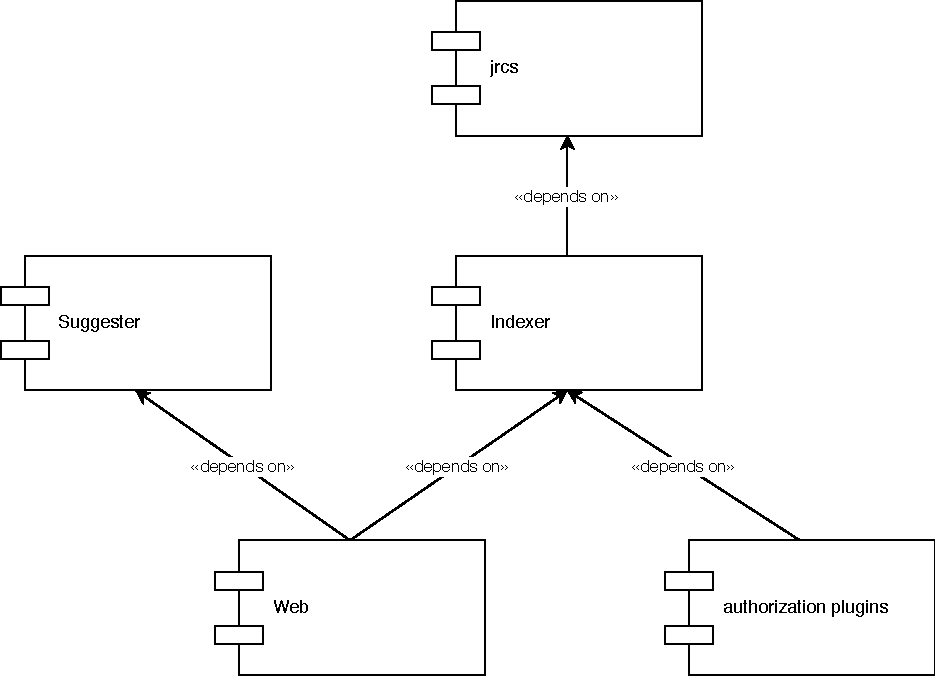
\includegraphics[width=100mm]{../img/opengrok_modules_changed.pdf}
    \caption{OpenGrok modules with Suggester module}
    \label{opengrok_modules_changed_img}
    \end{figure}
    \item \textbf{Implement suggester as a separate service} – this is a step towards microservices architecture
    \footnote{\url{https://en.wikipedia.org/wiki/Microservices}}. The suggester would run as a separate program
    listening on different port and possibly on different machine. Therefore; the implementation could be in any
    programming language and not necessarily in Java. Also, this could enable easy scalability of this service,
    e.g. one service per project. However, the suggester would still need access to the index files.
\end{itemize}

\textbf{Chosen solution} – in the end, the second proposal was chosen. Implementing suggester as a separate module is a
good compromise between a separate service and implementing it in the Web module. The main reason for this choice was that
OpenGrok does not support installation or scalability across multiple machines and these features are not planned to be
implemented in the near future. Therefore, it could be hard for users to set up and configure this new service.
However, suggester module needs to have public API and does not depend on any other OpenGrok modules. Therefore, it
will not require a lot of changes to bundle it as a separate service if the need arises in the future.

\section{OpenGrok Modifications}
\label{opengrok_modifications}

As discussed in \ref{general_architecture}, Suggester is added as a separate module which is a dependency of the
OpenGrok Web module. Therefore, changes to the Web module are required. OpenGrok uses Maven module structure.
Thus, Suggester module has to respect it as well.

\subsection{Frontend}

As described in \ref{opengrok-web} section, OpenGrok provides web interface. Some parts of the web need to be modified
for Suggester support.

\subsubsection{Configuring suggester}
OpenGrok provides configuration REST API endpoint for querying or manipulating the configuration of the Web application.
This endpoint could be used to retrieve the suggester configuration and apply it.
However, this endpoint is only reachable from the targeted machine because of the security reasons.
Therefore, it is needed to bypass this and provide one endpoint which will return only the suggester configuration.
This endpoint could also filter the information which is redundant to the JavaScript implementation.

\subsubsection{Showing the suggestions}
\label{showing_suggestions}

Suggester needs to detect if user pressed a key while having selected a specific input for which it is enabled. Upon
detecting this change it needs to process the data, send it to the backend part of the software, processs the returned
result and show it to
the user. All this should be as quick as possible so the user considers it to be seamless. Simplified picture of the
steps that need to be taken is shown on the figure \ref{suggest_sequence}.

\begin{figure}[htbp]
\centering
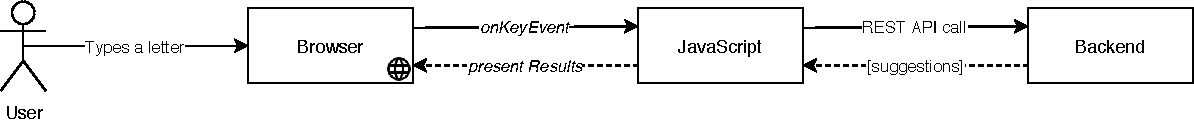
\includegraphics[width=145mm]{../img/opengrok_sequence.pdf}
\caption{Typical suggestions workflow}
\label{suggest_sequence}
\end{figure}

There are many libraries which provide "JavaScript" functionality as shown on figure \ref{suggest_sequence},
the most notable are:
\begin{itemize}
    \item jQuery UI Autocomplete\footnote{\url{https://jqueryui.com/autocomplete/}}
    \item Ajax Autocomplete for jQuery\footnote{\url{https://www.devbridge.com/sourcery/components/jquery-autocomplete/}}
    \item MagicSuggest\footnote{\url{http://nicolasbize.com/magicsuggest/}}
\end{itemize}

All of the above require jQuery\footnote{\url{http://jquery.com}} library which is already included in the OpenGrok.
In the end, jQuery UI Autocomplete was chosen because jQuery UI was already used by OpenGrok. Although, Autocomplete
module was not included. jQuery UI Autocomplete provides an easy-to-use API and is easily customizable, these factors
also contributed to the decision of picking this library.

\paragraph{Data format}
As mentioned, user's input must be sent to the backend part of the software, processed and
returned back. jQuery UI Autocomplete supports JSON\footnote{\url{https://www.json.org}} format by default. This format
is widely used and performs better than XML in this
specific situation (\url{https://www.w3schools.com/js/js_json_xml.asp}). Also OpenGrok's REST API supports
automatic conversion to JSON objects via the Jackson\footnote{\url{https://github.com/FasterXML/jackson}} library.
Therefore, it is a solid choice.

\subsubsection{Detecting the token for suggestions}
As referenced in \ref{opengrok_usage}, it is possible to write multiple tokens into one \textit{input} HTML tag.
Imagine the text: "car engine". With only this information the Suggester is not able to tell if it should add
suggestions for "car" prefix or "engine" prefix or something totally different. Therefore, the Suggester also requires the position of the last typed
key.

The position needs to be retrieved and set by the JavaScript part of the web page. This functionality could be written in
pure JavaScript; however, simple, small, and easy-to-use library jQuery caret (\url{https://github.com/acdvorak/jquery.caret})
was used instead.

\subsection{Backend}
As stated in \ref{showing_suggestions}, the server part needs to have a service which returns results based on the
input written by the user to the web page. And as mentioned in \ref{opengrok-web}, Web module is a web application compliant with
servlet API, therefore; new servlet which listens to the user's input and returns suggestions needs to be added.

\subsubsection{How to implement the suggester servlet}
The servlet represents a simple REST API endpoint
because it needs to respond to HTTP GET requests and return the response in JSON.
There is a lot of options how this could be achieved; however, the most notable are:
\begin{itemize}
    \item Use default implementation by extending \textit{HttpServletRequest} and its method \textit{doGet()}. The main
    advantage of this approach is that there are no other dependencies because they are provided by the underlying servlet container.
     However, some boilerplate code would need
    to be written which could be avoided.
    \item Use JAX-RS API and its implementation Jersey\footnote{\url{https://jersey.github.io}}. With this approach the
    result code could be clean and much easier to understand because of the use of provided annotations from JAX-RS API.
    Not to mention that Jersey provides additional features:
    \begin{itemize}
        \item Dependency injection.
        \item Bean validation support.
        \item Automatic JSON conversion using Jackson library.
    \end{itemize}
\end{itemize}

Since OpenGrok Web has already REST API support and both JAX-RS API and Jersey already on the classpath,
there is no dependency overhead. As a result, the second option was chosen.

\subsubsection{Processing user input}
\label{processing_user_input}
As referenced in \ref{opengrok_usage}, OpenGrok web interface provides multiple of HTML \textit{input} fields which
represent different Lucene \textit{fields} which should be searched. Each of these input fields can contain some value.
Therefore, all these values are passed to the server along with the information of currently selected input field and
the caret position in it.

Each of these fields can include any form of Lucene query, as stated in \ref{opengrok_usage}. Since these queries might
get very complicated, proper parser is needed. Lucene has a good support for this, which is also leveraged in OpenGrok
which has custom query parser which is almost identical to the one served by Lucene. However, character position is
useless after the parsing is done – it is not possible to find the token it referenced anymore. Therefore, a small
trick will be used. Before parsing the text data, a short, random but regarding the text unique, string of characters
is generated and inserted at the mentioned position. From now on, it is possible to use just this identifier since it
uniquely identifies the token in which the user is currently interested. However, this has also a small disadvantage.
If the query typed by the user is not correct then Lucene's parser generates \textit{ParseException} which contains
this identifier; therefore, it might be a little harder to decode the original query from the exception's message.

\subsubsection{Reacting to the Events}

Running OpenGrok Web instance has REST API which allows Indexer or administrators to indicate that some event occurred.
More information can be found at \ref{opengrok_rest}. Events that the suggester should be able to react to:
\begin{itemize}
    \item \textbf{Configuration change} – \textit{PUT /api/v1/configuration}

    Suggester should rebuild to be in concordance with the new configuration.
    \item \textbf{Indication to refresh index searchers} – \textit{PUT /api/v1/system/refresh}

    Most of the time this message indicates that the reindex of the data was done. Suggester
    should update its data to be up to date.

    \item \textbf{Marking project as indexed} – \textit{PUT /api/v1/projects/{project}/indexed}

    OpenGrok can know of projects which are not yet indexed. It is not possible to search in these projects;
    therefore, there is no need for suggester to know about them. However, this changes if the project is marked as indexed.
    Suggester should then build its inner data to support suggestions for the project.

    \item \textbf{Project delete} – \textit{DELETE /api/v1/projects/{project}}

    Suggester should drop any data it has regarding the project.
\end{itemize}

\section{Suggester}
\label{suggester_module}
This section looks at the Suggester module in more detail. First of all, it describes all the queries the suggester supports.
Then, looks at the fuzzy and boost factors. After that, discusses how to leverage previous searches. At last, mentions some
additional properties that were needed by this module.

\subsection{Prefix Query}
\label{prefix_query}
To start with, let's look at the simplest and at the same time probably the most used case. \textbf{Prefix query} is a special case of
\textit{Wildcard query} \ref{wildcard_query}. % TODO: add ref?
It can be divided into 2 parts:
\begin{itemize}
    \item \textbf{prefix} – text which represents the prefix of all the terms this query accepts.
    \item \textbf{*} – wildcard symbol which accepts any text (even zero-length text).
\end{itemize}

These parts are then combined together as: \textit{\{prefix\}*}.
It is probably the most used case because of the suggester nature. If user types any simple text (even without \textit{*}) then
the suggester automatically appends \textit{*} to the end and considers this as a prefix query to provide adequate suggestions.

Since prefix queries will be used that often then the suggester needs to be optimized for this type of queries.

\subsubsection{Scoring}
\label{prefix_scoring}
Every term needs to have a \textit{score} associated with it so the suggester could decide which term is better suited
to appear as a suggestion. Therefore, the problem is not only to find the terms with a specific prefix but to find $n$
terms with the best scores having the specific prefix. Let's assume that the suggester does not have any information
about previous searches. This case is discussed in
\ref{previous_searches}. The suggester has access to the Lucene index provided by the Indexer. % TODO: add refs?
Therefore; it has access to:
\begin{itemize}
    \item \textbf{Total term frequency $T$} – how many times the term appears in the document set.
    \item \textbf{Document frequency $N$} – in how many documents does the term appear.
    \item \textbf{Number of documents $D$} – total number of documents in the document set.
\end{itemize}

\paragraph{IDF\protect\footnote{\url{https://en.wikipedia.org/wiki/Tf\%E2\%80\%93idf\%23Inverse\_document\_frequency\_2}}}
At a first glance, it might seem a good idea to use inverse document frequency as a metric. The formula for computing this metric can be seen at \ref{IDF_eq}.
\begin{equation}
\label{IDF_eq}
IDF(t) = \log{\frac{D}{N}}
\end{equation}
Basically, it says how important is the term in the document set. If the term occurrs in every document then it is probably
a very common word and if provided in query it does not reduce the result set.
However, this importance is correct if the term is
provided by the user in the query. If the suggester were to use it, then it would suggest terms that are used the least, e.g. only once.
Therefore; this is not a good scoring option.

\paragraph{Document frequency}
Document frequency is a good indicator of how the term is used throughout the document set. However,
this metric is specific to the project. Thus, it would be hard to compare values across multiple projects. The solution
to the problem is normalization. Resultant equation can be seen at \ref{norm_doc_freq}.
\begin{equation}
\label{norm_doc_freq}
score = \frac{N}{D} \cdot constant
\end{equation}
This metric gives results which are expected of the suggester; therefore, it is the best option so far.

% TODO: find some work on this?

\subsubsection{Possible implementations}
\label{possible_implementations}
As mentioned before, the implementation should be fast to be able to fulfill the users' expectations. Although, at the
same time, it should not waste memory resources. One data structure per Lucene field per project is needed. The OpenGrok
installation can contain hundreds of projects and depending on the size of the project, one Lucene field can possibly contain
tens of thousands of terms or even more (in some cases millions).

\paragraph{Trie\protect\footnote{\url{https://en.wikipedia.org/wiki/Trie}}} – sometimes called prefix tree, is the simplest
structure suitable for our purposes. However, it does not support efficient lookup based on scores. It would
be needed to traverse the whole subtree for a specific prefix to find the terms with the best scores.

\paragraph{Ternary search tree\protect\footnote{\url{https://en.wikipedia.org/wiki/Ternary\_search\_tree}}} – is a
special case of a Trie. Same as Trie, it does not have any support for more efficient lookup based on scores.

\paragraph{FST\protect\footnote{\url{https://en.wikipedia.org/wiki/Finite-state\_transducer}}} \label{FST} – is a finite state
automaton which can produce output. Special case of FST is a weighted FST (WFST) where each transition can have an
associated weight. It is possible to construct a WFST which will provide a very efficient algorithm for finding the
$n$ terms with the best scores. This algorithm is explained in \citep{Mohri02anefficient}. However, this algorithm returns
terms with the lowest scores and based on the chosen scoring it is needed for it to return the terms with the highest
scores. This can be achieved by a neat trick, it is possible to invert the score by the formula \ref{invert_score}.
\begin{equation}
\label{invert_score}
newScore = maxPossibleScoreValue - score
\end{equation}
An efficient construction of minimal, acyclic and deterministic WFST is explained in \citep{Mihov01directconstruction}.

\textbf{Example} – WFST with terms and weights: $CAR = 10, CARS = 15, CART = 5$ can be seen on \ref{wfst_example}.

\begin{figure}[htbp]
\centering
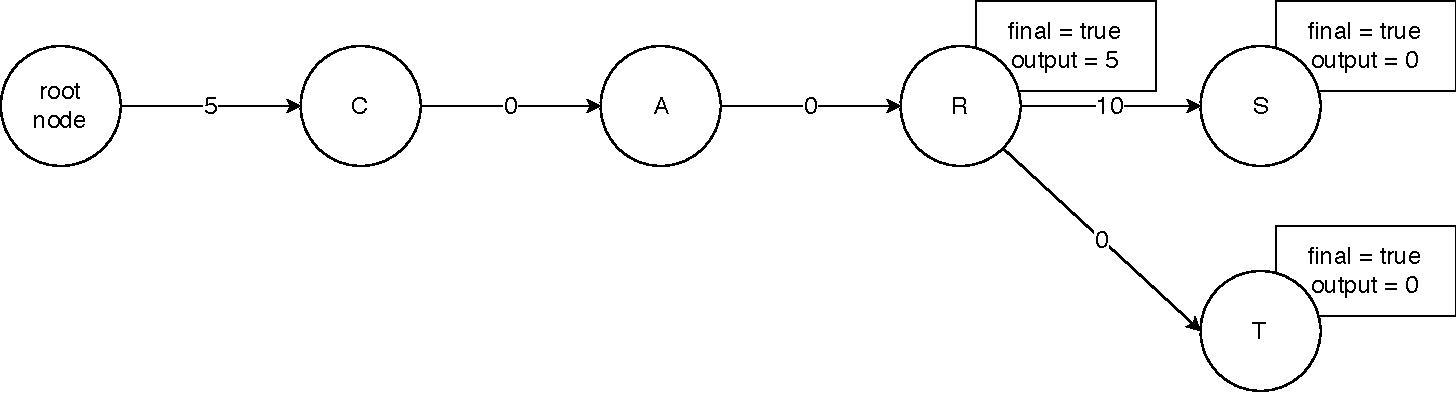
\includegraphics[width=145mm]{../img/wfst.pdf}
\caption{WFST example}
\label{wfst_example}
\end{figure}

% TODO: describe algorithm?

\paragraph{Comparison}

Two kinds of dataset were used:
\begin{itemize}
    \item \textbf{English words} – list of \textbf{370099} words freely available at \url{https://github.com/dwyl/english-words}.
    \item \textbf{Linux kernel} – \textit{full} field of indexed Linux kernel with \textbf{3459733} terms.
\end{itemize}

% TODO: useful info average term length in Linux kernel: 22.033919380483987

Measured was average time of specific operations on the data structures.
Description of the test cases:
\begin{itemize}
    \item \textbf{"non" Prefix Lookup} – is a lookup of 10 words with the prefix "non" which is the most occurring prefix
    of length 3 in the English words dataset with 7479 occurrences. Linux kernel has only 644 occurrences. Results can be seen
    on graph \ref{comp_non}.

    \begin{figure}[htbp]
        \centering
        \begin{tikzpicture}
            \begin{axis}[
                ybar,
                bar width=20pt,
                xlabel={Dataset},
                ylabel={Time (seconds)},
                ymin=0,
                ytick=\empty,
                xtick=data,
                axis x line=bottom,
                axis y line=left,
                enlarge x limits=0.2,
                symbolic x coords={Linux kernel, English words},
                xticklabel style={anchor=base,yshift=-\baselineskip},
                nodes near coords={\pgfmathprintnumber\pgfplotspointmeta}
            ]
            \addplot[ybar, fill=white, error bars/.cd, y dir=both, y explicit] plot coordinates {
            (English words, 0.0001)
            (Linux kernel, 0.00001)
            };

            \addplot[ybar, fill=gray, error bars/.cd, y dir=both, y explicit] plot coordinates {
            (English words, 0.00001)
            (Linux kernel, 0.00001)
            };
            \legend{TST, WFST}
            \end{axis}
        \end{tikzpicture}
        \caption{"non" Prefix Lookup comparison}
        \label{comp_non}
    \end{figure}
    \item \textbf{One Letter Prefix Lookup} – is a lookup of 10 words with the prefix of each letter from the basic alphabet.
    Results can be seen on graph \ref{comp_one}.

    \begin{figure}[htbp]
        \centering
        \begin{tikzpicture}
            \begin{axis}[
                ybar,
                bar width=20pt,
                xlabel={Dataset},
                ylabel={Time (seconds)},
                ymin=0,
                ytick=\empty,
                xtick=data,
                axis x line=bottom,
                axis y line=left,
                enlarge x limits=0.2,
                symbolic x coords={Linux kernel, English words},
                xticklabel style={anchor=base,yshift=-\baselineskip},
                nodes near coords={\pgfmathprintnumber\pgfplotspointmeta}
            ]
            \addplot[ybar, fill=white, error bars/.cd, y dir=both, y explicit] plot coordinates {
            (English words, 0.029) += (English words, 0.001) -= (English words, 0.001)
            (Linux kernel, 0.344) += (Linux kernel, 0.006) -= (Linux kernel, 0.006)
            };

            \addplot[ybar, fill=gray, error bars/.cd, y dir=both, y explicit] plot coordinates {
            (English words, 0.001) += (English words, 0.001) -= (English words, 0.001)
            (Linux kernel, 0.001) += (Linux kernel, 0.001) -= (Linux kernel, 0.001)
            };
            \legend{TST, WFST}
            \end{axis}
        \end{tikzpicture}
        \caption{One Letter Prefix Lookup comparison}
        \label{comp_one}
    \end{figure}

    \item \textbf{Two Letter Prefix Lookup} – is a lookup of 10 words with the prefix which is a combination of 2 letters
    from the basic alphabet. Results can be seen on graph \ref{comp_two}.

    \begin{figure}[htbp]
        \centering
        \begin{tikzpicture}
            \begin{axis}[
                ybar,
                bar width=20pt,
                xlabel={Dataset},
                ylabel={Time (seconds)},
                ymin=0,
                ytick=\empty,
                xtick=data,
                axis x line=bottom,
                axis y line=left,
                enlarge x limits=0.2,
                symbolic x coords={Linux kernel, English words},
                xticklabel style={anchor=base,yshift=-\baselineskip},
                nodes near coords={\pgfmathprintnumber\pgfplotspointmeta}
            ]
            \addplot[ybar, fill=white, error bars/.cd, y dir=both, y explicit] plot coordinates {
            (English words, 0.029) += (English words, 0.002) -= (English words, 0.002)
            (Linux kernel, 0.323) += (Linux kernel, 0.004) -= (Linux kernel, 0.004)
            };

            \addplot[ybar, fill=gray, error bars/.cd, y dir=both, y explicit] plot coordinates {
            (English words, 0.006) += (English words, 0.001) -= (English words, 0.001)
            (Linux kernel, 0.014) += (Linux kernel, 0.001) -= (Linux kernel, 0.001)
            };
            \legend{TST, WFST}
            \end{axis}
        \end{tikzpicture}
        \caption{Two Letter Prefix Lookup comparison}
        \label{comp_two}
    \end{figure}

    \item \textbf{Build time} – performs build of the data structure from the scratch. Results can be seen on graph
    \ref{comp_build}.

    \begin{figure}[htbp]
        \centering
        \begin{tikzpicture}
            \begin{axis}[
                ybar,
                bar width=20pt,
                xlabel={Dataset},
                ylabel={Time (seconds)},
                ymin=0,
                ytick=\empty,
                xtick=data,
                axis x line=bottom,
                axis y line=left,
                enlarge x limits=0.2,
                symbolic x coords={Linux kernel, English words},
                xticklabel style={anchor=base,yshift=-\baselineskip},
                nodes near coords={\pgfmathprintnumber\pgfplotspointmeta}
            ]
            \addplot[ybar, fill=white, error bars/.cd, y dir=both, y explicit] plot coordinates {
            (English words, 0.433) += (English words, 0.01) -= (English words, 0.01)
            (Linux kernel, 13.264) += (Linux kernel, 1.978) -= (Linux kernel, 1.978)
            };

            \addplot[ybar, fill=gray, error bars/.cd, y dir=both, y explicit] plot coordinates {
            (English words, 0.706) += (English words, 0.003) -= (English words, 0.003)
            (Linux kernel, 17.296) += (Linux kernel, 0.12) -= (Linux kernel, 0.12)
            };
            \legend{TST, WFST}
            \end{axis}
        \end{tikzpicture}
        \caption{Comparison of build times}
        \label{comp_build}
    \end{figure}


    \item \textbf{Memory usage} – approximate sizes the data structures use in the computer's main memory.
     The result can be seen on graph \ref{comp_mem}. The data was measured by calling method
     \textit{ramBytesUsed()} which is a custom method commonly implemented in Lucene's data structures.
     The drastic
    difference is mainly due to WFST's implementation which was optimized to use as little memory as possible while
    providing a very solid performance. Some of the WFST' optimizations:
    \begin{itemize}
        \item Storage in byte arrays. There is no need to keep references to the objects which take 8B on 64-bit computer
        but rather smaller identifiers. Also, differences in arc weights are mostly very small. The implementation
        leverages this and encodes integers with variable length into the mentioned byte arrays.
        \item Caching of the first arcs of the FST.
        \item Constant arc size for the arcs into certain depth which allows binary search among the arcs. (Random
        access is not possible because it would require more memory which would not be used.)
    \end{itemize}
    It can be noted that some of these optimizations may hinder the performance. However, the result seems to be a good
    compromise.

    \begin{figure}[htbp]
        \centering
        \begin{tikzpicture}
            \begin{axis}[
                ybar,
                bar width=20pt,
                xlabel={Dataset},
                ylabel={Memory usage (MiB)},
                ymin=0,
                ytick=\empty,
                xtick=data,
                axis x line=bottom,
                axis y line=left,
                enlarge x limits=0.2,
                symbolic x coords={Linux kernel, English words},
                xticklabel style={anchor=base,yshift=-\baselineskip},
                nodes near coords={\pgfmathprintnumber\pgfplotspointmeta}
            ]
            \addplot[ybar, fill=white, error bars/.cd, y dir=both, y explicit] plot coordinates {
            (English words, 68.4622154236)
            (Linux kernel, 1226.1035423279)
            };

            \addplot[ybar, fill=gray, error bars/.cd, y dir=both, y explicit] plot coordinates {
            (English words, 3.8268890381)
            (Linux kernel, 21.9446716309)
            };
            \legend{TST, WFST}
            \end{axis}
        \end{tikzpicture}
        \caption{Comparison of memory usage}
        \label{comp_mem}
    \end{figure}

\end{itemize}

How to reproduce these benchmarks and description of the machine on which they were run can be found in \ref{benchmark_attachment}.

Based on the provided results it can be noticed that WFST performs much better at lookups. Mainly at lookups with a short prefix.
Also, the memory usage is inarguably better in WFST data structures. However, its build time is worse by a small margin than TST's.

OpenGrok installation can easily contain dozens of projects, each of these projects contains 5 Lucene fields
(full, defs, refs, path, hist) which needs to have suggester support. Depending on the size of the projects,
TST implementation could take many GiBs of the memory which is not feasible.

To conclude, WFST is a better option in almost every aspect except the build time which is not that important because of
the possibility of saving the data structures on the disk; and therefore, avoid it almost every time except when the index changes.

\subsection{Wildcard Query}
\label{wildcard_query}
The specific case of \textit{prefix*} is covered in the previous section \ref{prefix_query}. Therefore, in this section
will be covered all the other cases of wildcard queries. The implementation of WFST cannot be used because its nature.
There is no way how to efficiently find in WFST tokens for the query of type \textit{*sufffix}. The required result is
the same as for prefix query: to find the terms which are accepted by the query with the top score. However, the data
structure which could achieve this for generic wildcard query with the WFST performance is not known to the author.
Nonetheless, the Lucene evaluation of wildcard queries could be leveraged. Automaton specific to the wildcard query is
created and then the terms are filtered using this automaton. The implemenation is slower as WFST because all the terms
needs to filtered once if they are accepted by the automaton then they need to be filtered for the second time based on
their score.

\subsubsection{Scoring}
Scoring used is the same as mentioned in \ref{prefix_scoring}.

\subsection{Regular Expression Query}
The regular expression queries can be implemented in the same way as wildcard queries \ref{wildcard_query}. The only difference
is that the automaton is created based on the regular expression rules.

\subsection{Phrase Query}
\label{suggest_phrase_query}
Phrase query is a query which specifies a collection of tokens which must occur in the documents in the specified order.
The tokens must be surrounded by double quotes, e.g. \textit{"token1 token2"}. In this example, this means that \textit{token1} must be immediately followed by
\textit{token2} in the document for it to be accepted.

\subsubsection{Evaluation}
\label{prefix_evaluation}
As mentioned in \ref{indexer:index},
Lucene stores data in reverse document index. However, to be able to determine if one token is immediately followed by another
token, their position needs to be stored and accessed. Lucene can be configured to store this information as well.
It can be easily determined if Lucene stored this data by checking if Lucene index contains a file with a \textit{.pos}
suffix.

Evaluation of the query is straightforward. Lucene performs lookup for each token in the phrase query and intersects the
results which provides all the documents which contain all of these tokens. Then it checks if the tokens are indeed
next to each other and on correct positions.

\subsubsection{Getting the suggestions}
\paragraph{Using shingles}
Shingle\footnote{\url{https://en.wikipedia.org/wiki/W-shingling}} is an n-gram of words. It would be possible to create
shingles of specific count (e.g. 2 to 5 words) during the indexing phase. Each shingle would be treated as a single term.
Then, it would be possible to do quick prefix lookup as described in \ref{prefix_query}. However, this solution has many drawbacks:
\begin{itemize}
    \item Another, not quite small index would have to be created.
    \item The suggestions would work for only the last token of the phrase query.
    \item The maximum number of tokens in phrase query for which the suggestions would work would be limited by the longest
    shingle.
    \item Another data structure which would contain all of the shingles for quick lookup would have to be stored in the
    main memory.
\end{itemize}

\paragraph{Using the default evaluation}
As explained in \ref{processing_user_input}, it is known which token should be considered as prefix. Therefore, this token
can be omitted but the requested position of other tokens must stay unchanged. Then the same evaluation as mentioned in
\ref{prefix_evaluation} can be used. The result of the evaluation is a pair:
\begin{itemize}
    \item Document identifier.
    \item Token position.
\end{itemize}
Based on this information it should be possible the gather all the possible terms and accept only those with the
provided prefix.

\paragraph{Getting the token at specific position}
Based on the document identifier and token position it should be easy to get the needed term. However, Lucene does not
provide any functionality how to do this efficiently because the nature of the reverse document index is a complete
opposite to the data structure which would provide efficient implementation of this operation. Possible solutions are:
\begin{itemize}
    \item Implement data structure which would efficiently lookup a term based on a position and document identifier.
    However, the size of the data structure would not be trivial in comparison with the actual index size. Furthermore,
    it would slow down the indexing phase even more which might already take a few hours or even days if the projects
    being indexed are very huge.
    \item Read and tokenize the document with the specified identifier. Nonetheless, this might be a slow operation if there
    was a lot of documents accepted by the query because of the necessary
    I/O\footnote{\url{https://en.wikipedia.org/wiki/Input/output}} operations.
    \item Use the already existing reverse document index. It is possible to lookup all the terms based on the prefix.
    Then filter the terms which do not occur in the documents which were found by the phrase query and those which
    do not have correct position in the document.
\end{itemize}

The first option is not feasible because of the added size to the already existing index. Comparison between the
second and the third option can be found in the table ...

% TODO: add table

Based on the results in ... it is clear that ...

\subsubsection{Scoring}
It would be possible to use the same scoring as in \ref{prefix_scoring}. However, the scoring is not specific enough.
For instance, the term could have a big document frequency but in the context of phrase query would occur only once,
whereas, the term with lower document frequency could occur more times, which would make it more specific. Therefore,
the scoring based on the term frequency in the context of phrase query provides better results.

\subsection{Range Queries}
Range queries have many similarities with wildcard queries \ref{wildcard_query} in terms of implementation for the
suggester. The main difference is in creation of the automaton. Range query contains lower and upper term. The
suggestions depends on which of the terms is used as a prefix.

\subsubsection{Lower Term as a Prefix}
First of all, the automaton $A_{int}$ which represents a binary interval is created between the lower and upper term. Then,
automaton $A_{prefix}$ which accepts all terms with prefix specified in the lower bound is needed. The result automaton is the
intersection of these two, as in \ref{lt_automaton}.

\begin{equation}
\label{lt_automaton}
A_{result} = A_{int} \cap A_{prefix}
\end{equation}

\subsubsection{Upper Term as a Prefix}
Similarly, the automaton $A_{prefix}$ which accepts all terms with prefix specified in the upper bound is created. Then,
another binary interval automaton $A_{int}$ is needed; however, this one has no lower bound specified and for upper bound the
lower term of the query is used. The result automaton needs to be created as a difference between the prefix automaton
and the binary interval automaton, as in \ref{ut_automaton}.

\begin{equation}
\label{ut_automaton}
A_{result} = A_{prefix} - A_{int}
\end{equation}

\subsection{Including Boolean Operators}
\label{boolean_ops}

% TODO: probably move this to OpenGrok chapter, this chapter should be about suggester

There are multiple boolean operators which can modify the meaning of the term in the query.

\subsubsection{Unary Boolean Operators}
Following unary operators are supported:
\begin{itemize}
    \item \textbf{+} unary operator in front of the term means that the term must occur in the result document set.
    \item \textbf{-} unary operator in front of the term means that the term cannot occur in the result document set.
    It is also possible to use synonyms \textbf{NOT} or \textbf{!}. However, it is not possible to use it in a query
    with a single term.
    \item \textbf{Default} unary operator – no unary operator in front of the term means that the term should occur
    in the result document set.
\end{itemize}

\subsubsection{Binary Boolean Operators}

At first, let's look at the simple case with only one binary boolean operator and two terms, as in \ref{simple_boolean_op}.

\begin{equation}
\label{simple_boolean_op}
term1\ \diamondsuit \ term2
\end{equation}

If the $\diamondsuit$ is:
\begin{itemize}
    \item \textbf{AND} – or $\&\&$, is rewritten as in \ref{simple_and_op}.
    \begin{equation}
    \label{simple_and_op}
    +term1\ +term2
    \end{equation}
    \item \textbf{OR} – or $\vert\vert$, is rewritten as in \ref{simple_or_op}. (Default unary operators are used.)
    \begin{equation}
    \label{simple_or_op}
    term1\ term2
    \end{equation}
\end{itemize}

\paragraph{Multiple binary operators}
It is possible to use multiple binary operators as in \ref{multiple_boolean_op}.

\begin{equation}
\label{multiple_boolean_op}
term1\ \diamondsuit \ term2\ \diamondsuit \ … \ \diamondsuit \ termN
\end{equation}

However, there is no operator precedence (\textit{AND} and \textit{OR} have the same precedence). Therefore, without grouping
(described in \ref{grouping_queries}) it might
not be clear what unary operator (default or +) will be assigned to the middle terms.
Lucene parses the query sequentially from left to right and upon encountering the binary operator changes the surrounding terms. For instance,
query as in \ref{boolean_query_example} will be transformed to \ref{boolean_query_res}.

\begin{equation}
\label{boolean_query_example}
a\ \&\&\ b\ \vert\vert\ c\ \&\&\ d\ \vert\vert\ !e
\end{equation}

\begin{equation}
\label{boolean_query_res}
{+}a\ b\ {+}c\ d\ {-}e
\end{equation}

\subsubsection{Suggester}
The suggester can be interested only in unary boolean operators because binary boolean operators are transformed into unary.
Let's assume query with multiple terms. One of those terms is a prefix for which the suggester needs to provide suggestions.
Based on the unary operator the prefix has assigned, the suggester needs to:
\begin{itemize}
    \item \textbf{+} – the suggested term must occur in the result set. Therefore, it is dependent on the other terms.
    For instance, if the query contains another term which must occur in the result set, then the suggester should only
    suggest the terms which are occurring in the same documents as the term. If it did not, then user could be easily
    confused and the result set might be empty. The solution to this problem is to:
    \begin{enumerate}
        \item Extract the prefix term from the query.
        \item Get all the documents that satisfy the bare query.
        \item Suggest only terms which occur in at least one of the retrieved documents in step 2.
    \end{enumerate}
    \item \textbf{default} – the suggested term should occur in the result set. However, if it does not then nothing is broken.
    Nevertheless, suggesting terms that cannot appear in the result document set does not make much sense. Thus, it is performed
    as in \textit{+} unary operator.
    \item \textbf{-} – the suggested term must not appear in the result set and as mentioned, it cannot be used in a
    query with a single term; therefore, it's purpose is to reduce the result set. Thus, the same solution as for \textit{+}
    needs to be performed.
\end{itemize}

\paragraph{Scoring}
The scoring should follow the same principle as in \ref{prefix_scoring} because of the consistency. However,
the document frequency has to be taken from the result set of the bare query and not the whole index.

\subsection{Grouping Queries}
\label{grouping_queries}
With boolean operators (\ref{boolean_ops}) it is possible to create complex queries. However, it is not possible to
combine queries in an easy manner. That's where grouping operators \textbf{(} and \textbf{)} has their use. For instance,
it is possible to combine results of two queries as can be seen in \ref{grouping_query}.

\begin{equation}
\label{grouping_query}
(query1)\ \vert\vert\ (query2)
\end{equation}

It is also possible to use grouping operators to remove the confusion caused by the omition of precedence for the binary
boolean operators. Therefore, it is possible to write queries as shown in \ref{grouping_query2}.

\begin{equation}
\label{grouping_query2}
(term1\ AND\ term2)\ OR\ term3
\end{equation}

Grouping operators can be nested, thus; it is easy to create truly complex queries.

\subsubsection{Suggester}

At first, the query is parsed into multiple simple queries which are then combined together to create one complex
\textit{BooleanQuery}. It is possible to imagine the top-down decomposition into tree-like structure. % TODO: add images
One leaf is the suggester query. This clause is marked and replaced by \textit{MatchAllDocsQuery} which matches every
document. % TODO: add explanation
It is possible to start at this leaf and go towards the root. On each node on the path towards the root there may be
multiple clauses. The algorithm looks at all clauses and removes the clauses which have specified \textit{SHOULD}
occurrence. The clause in which the suggester query resides is preserved by default. When the algorithm ends the result
is a stripped query which contains only queries that affect the suggestions.

\subsection{Dealing with fuzzy factor}
It is possible to specify a fuzzy factor for the queries which indicates how well should the query match the documents.

\subsubsection{Fuzzy search}
Lucene supports fuzzy searches which are based on the Levenshtein Distance
\footnote{\url{https://en.wikipedia.org/wiki/Levenshtein_distance}} algorithm. This option can be specified by typing
$\sim$ after the searched term and followed by the value of the fuzzy factor. However, it can be only specified for the
single term query. Suggester supports this option. By writing the $\sim$ with the fuzzy factor after the term the
suggester will suggest the terms which satisfy this condition.

\subsubsection{Proximity search}
Proximity search is a phrase query with specified fuzzy value. The fuzzy value represents the allowed edit distance of the
tokens of the phrase query. The implementation is very similar to \ref{suggest_phrase_query}. However, the suggestions
take the fuzzy factor into account and will contain terms that satisfy this condition.

\subsection{Dealing with boost factor}
Lucene supports term boosting by writing \textbf{\^} after the searched term and followed by the value of the boost factor.
Default boost factor is 1. It must be positive but can be less than 1. The boost factor specifies how is the term relevant
in regard to other terms. In a query \ref{boost} the term \textit{term1} is more relevant then the term \textit{term2}.

\begin{equation}
\label{boost}
term1\ \hat{}\ 3\ \&\&\ term2
\end{equation}

It might be possible for complex queries to take this information and boost those suggested terms that are in the same
document as boosted term. However, for now, the boost factor is ignored by the suggester.

\subsection{Promoting suggestions based on previous searches}
The \textbf{reciprocal rank} of a query response is the multiplicative inverse of the rank of the first correct answer.
That means, if the first correct answer was on the third place then reciprocal rank would be $\frac{1}{3}$.

\textbf{Mean reciprocal rank}\footnote{\url{https://en.wikipedia.org/wiki/Mean\_reciprocal\_rank}}(MRR) is defined as
average of reciprocal ranks for a set of queries $Q$. Mathematically, it is defined as in \ref{mrr}.

\begin{equation}
\label{mrr}
MRR = \frac{1}{\vert Q \vert} \sum_{i=1}^{\vert Q \vert} reciprocalRank_i
\end{equation}

In \citep{Bar-yossef11context-sensitivequery} are presented multiple approaches to the suggestions based on previous
searches:
\begin{itemize}
    \item \textbf{Most popular completion} – wisdom of the crowds. For some prefix the suggester suggests the terms
    with the same prefix that were searched the most.
    \item \textbf{Nearest completion} – takes into account current context of the user that is typing the queries.
    The authors defined \textbf{logical search session} as an interactive process in which the user (re-)formulates queries
    while searching for documents satisfying a particular information need. It consists of a sequence of
    queries $q_1, . . . , q_t (t \geq 1)$ issued by the user. The \textbf{context} of a user input $x$, where $x$ is the prefix of
    some query $q_i$ in the session, is the sequence of queries $q_1, . . . , q_{i-1}$ preceding $q_i$.
    Authors also specified how to convert context to a vector which can be used to find the most similar query.
    This works for vector model based search engines. Lucene is a combination of vector and boolean model so the
    conversion could be applicable.

    \item \textbf{Hybrid completion} – if there is no or almost no context then \textit{nearest completion} cannot predict the
    suggestions. Therefore, \textit{hybrid completion} is a combination of \textit{most popular completion} and \textit{nearest completion}.
    The authors have shown in empirical study that \textit{hybrid completion} has better \textit{MRR} than
    \textit{most popular completion} on average.
\end{itemize}


\textbf{Chosen solution} – \textit{nearest completion} and thus \textit{hybrid completion} are very intriguing and could
improve the suggestions by a big margin. However, they would need to be adapted to Lucene and the implementation
might not be completely straightforward. Therefore, the basic implementation of suggester will only include the
\textit{most popular completion}. Implementation of the \textit{nearest completion} is a very promising canditate for
future extensions.

\subsubsection{Most Popular Completion – Simple Queries}

To implement most popular completion the score of the terms needs to be changed by some factor. For instance, if the term
$term1$ was searched for $i$ times then the score could be changed by a number $h(i)$ for some function $h: \mathbb{N} \mapsto \mathbb{N}$.
It is also possible to take into account how recent the searches were and if there is a multiple recent searches for some
term then increase its score by a higher value. For instance, this could arise in a situation if some error was found in
method $m()$ of some well known library, then multiple users will probably be searching for it in a small time interval.
However, the suggester will focus only on basic implementation that considers only the term search count mainly because
its simplicity. Time factor is a possible extension to an existing solution.

It is needed to have a key-value store for storing the number of searches for the terms. This store should be persistent
so the data would not be lost after the restart of the application. Also this store should allow parallel access for
efficiency. There are multiple options how to achieve this functionality:
\begin{itemize}
    \item \textbf{Java Map} implementation with concurrent access, e.g. \textit{ConcurrentHashMap}. This map could be stored
    on the disk periodically to fulfil the persistency requirement. This solution has a few drawbacks:
    \begin{itemize}
        \item Loss of recent data after restart/crash.
        \item The data are held in memory. The size of the data is non-trivial, e.g.
        \textit{Linux kernel} dataset contained approximately $3.5 million$ terms for \textit{full} field.
    \end{itemize}

    \item \textbf{Redis}\footnote{\url{https://redis.io}} – in-memory data structure store, used as a database, cache
    and message broker. It has support for multiple languages and contains the needed commands (\textit{GET, INCR}).
    The major drawback is that Redis would have to be installed and run separately. Although some embedded Redis solutions
    exist, those are meant for testing purposes. Redis also has support for persistence:
    \begin{itemize}
        \item \textbf{RDB} persistence – performs point-in-time snapshots of the dataset at specified intervals.
        \item \textbf{AOF} persistence – logs every write operation received by the server, that will be played again
        at server startup, reconstructing the original dataset.
    \end{itemize}

    \item \textbf{Relational Database} – even though traditional databases satisfy most of the needs, they do not
    provide the sufficient speed performance.

    \item \textbf{Chronicle Map}\footnote{\url{https://chronicle.software/products/map/}} – provides a Java Map like
    interface and stores data off-heap. Data can be persistent by the use of memory mapped
    files\footnote{\url{https://en.wikipedia.org/wiki/Memory-mapped\_file}}. Disadvantages are that some hints are
    needed for the data structure to perform efficiently:
    \begin{itemize}
        \item Number of entries – can be overestimated. However, the authors specify that it would be best to specify
        this number to the actual number of entries stored $\pm 10\%$. Even though it is possible to store more elements
        than specified, the performance of the data structure decreases marginally.
        \item Average key size – does not affect maximum key size.
    \end{itemize}

    \item \textbf{MapDB}\footnote{\url{http://www.mapdb.org}} – similar to Chronicle Map but no hints are necessary.

    \item \textbf{LMDB for Java}\footnote{\url{https://github.com/lmdbjava/lmdbjava}} – Java mapping for
    LMDB\footnote{\url{https://symas.com/lmdb/}}. Major drawbacks:
    \begin{itemize}
        \item Low level API – keys and values need to be passed in byte buffers.
        \item Hints needed:
            \begin{itemize}
                \item Number of entries – can be overestimated.
                \item Maximum key size – must be the same as maximum term size in Lucene which 32767 bytes.
            \end{itemize}
    \end{itemize}

    Benchmark comparing MapDB, Chronicle Map, LMDB and some other solutions can be found here:
    \url{https://github.com/lmdbjava/benchmarks/blob/master/results/20160710/README.md}.

\end{itemize}

As mentioned in \ref{possible_implementations}, the best option for simple prefix queries is a WFST data structure.
Mainly because its low memory footprint and fast lookups.
Every term has assigned a score based on its occurrence frequency as mentioned in \ref{prefix_scoring}. This score
can be computed at the start and does not change very often – only after performing reindex.

The best and easiest solution would be to change term score in WFST directly. However, this is not possible because
Lucene's implementation of WFST is read-only. Let's examine possible modifications to WFST to allow changing score of the
terms.
\begin{itemize}
    \item WFST is stored in a byte array (\textit{byte[]}) or multiple byte arrays to allow low memory footprint. The
    arc values are very often small because they represent only difference to the smallest term in the subtree. Lucene
    implementation leverages this and for small values less bytes need to be written. For instance, take an \textit{int}
    data type, it needs 4 bytes to be stored properly. However, in WFST implementation it takes between 1 and 5 bytes.
    The smaller values need less space. Per byte, the highest order bit indicates whether the next byte is part of this
    number and the remaining 7 bits contain the actual value. Even though this allows for a very efficient memory requirements,
    the modifications are a problem. If we were to increase some value, then it might take more bytes than it actually has available.
    Therefore, part of the byte array would need to be shifted by 1 byte. This operation would prevent parallel access.
    One solution might be that there would be another array where the content would be copied and then the references
    would be swapped. However, this does not allow parallel modifications.
    Another solution is to discard the variable length of the values and allocate a constant size for them,
    e.g. 4 bytes for \textit{int}. This however increases memory footprint as can be seen on \ref{enc_comp}.

    \begin{figure}[htbp]
        \centering
        \begin{tikzpicture}
            \begin{axis}[
                ybar,
                bar width=20pt,
                xlabel={Dataset},
                ylabel={Memory usage (MiB)},
                ymin=0,
                ytick=\empty,
                xtick=data,
                axis x line=bottom,
                axis y line=left,
                enlarge x limits=0.2,
                symbolic x coords={Linux kernel, English words},
                xticklabel style={anchor=base,yshift=-\baselineskip},
                nodes near coords={\pgfmathprintnumber\pgfplotspointmeta}
            ]

            \addplot[ybar, fill=white, error bars/.cd, y dir=both, y explicit] plot coordinates {
            (English words, 3.8268890381)
            (Linux kernel, 21.9446716309)
            };

            \addplot[ybar, fill=gray, error bars/.cd, y dir=both, y explicit] plot coordinates {
            (English words, 4.6938095093)
            (Linux kernel, 41.9976768494)
            };

            \addplot[ybar, fill=black, error bars/.cd, y dir=both, y explicit] plot coordinates {
            (English words, 7.3886260986)
            (Linux kernel, 62.2045021057)
            };

            \legend{unmodified, modified – int, modified – long}
            \end{axis}
        \end{tikzpicture}
        \caption{Comparison of memory usage when changing number encoding}
        \label{enc_comp}
    \end{figure}

    The memory usage increased by approximately $22\%$ for \textit{English words} dataset. However, it can be
    almost doubled as can be seen on \textit{Linux kernel} dataset where approximately $92\%$ size increase can be noticed.
    The graph \ref{enc_comp} also shows the case when the encoding would use \textit{long} datatype. Although Lucene's \textit{Lookup}
    interface specificies \textit{long} datatype, WFST implementation supports only \textit{int} so far.

    \item Lucene's WFST implementation does not know the notion of nodes but the data are stored only in arcs. Arcs that
    start in the root node might be stored in memory directly and therefore are not encoded in byte array since these
    arcs are acessed very often
    and the decoding from byte array has an impact on the data structure lookup performance. Although this is not a big issue,
    the modifications would need to take this into account and add checks for this case.

    \item In some cases (e.g. the depth of an arc is less than a constant or there is more arcs from one node than
    another constant) the arcs
    might not be encoded as efficiently as possible but rather take a constant size. This then allows to do a binary
    search of arcs rather than going over them sequentially. Thus, increasing the speed of the lookup.

    \item As explained in \ref{FST}, scores of the terms are inverted (\ref{invert_score}) so by increasing score of some term
    we are actually decreasing its weight in WFST. Sum of arc values on the path to a term is the weight of the term (plus the final output modifier).
    However, the arc value tries to represent the lowest weight of the term in its subtree. And by decreasing this weight
    it could be necessary to update the whole WFST data structure. For instance, let's suppose that we have WFST as in \ref{wfst_example}
    and that the weight of the term $CAR$ will change to value $2$. The changes can be seen on the \ref{wfst_modified} in red color.

    \begin{figure}[htbp]
    \centering
    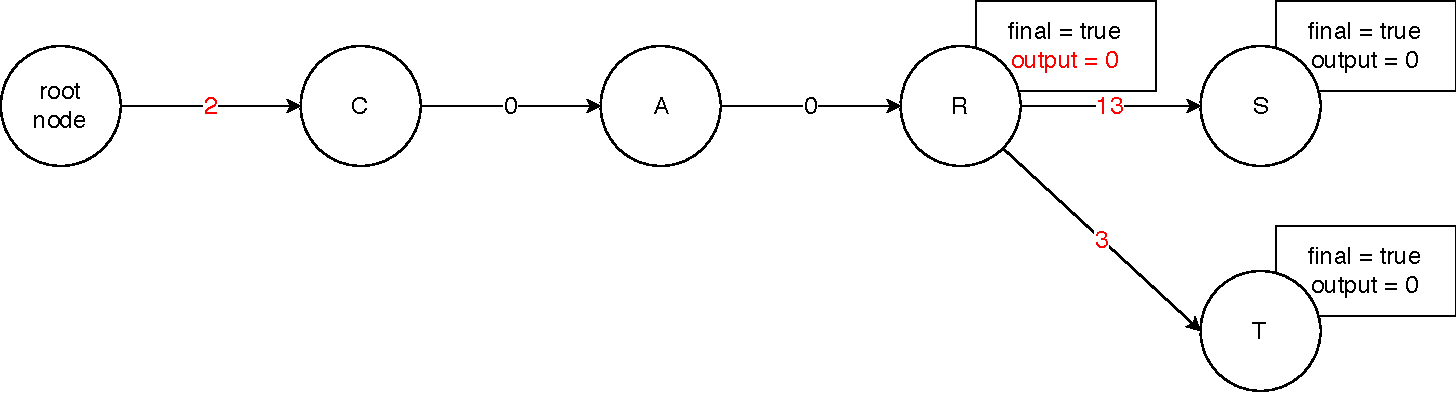
\includegraphics[width=145mm]{../img/wfst_modified.pdf}
    \caption{WFST modifications}
    \label{wfst_modified}
    \end{figure}

\end{itemize}

As a consequence of these observations, it was decided that modifying the WFST to allow changing scores could be a difficult
endeavour. Therefore, the remaining option was to rebuild WFSTs per some time interval. The most negative impact is that the
suggestions for simple queries will not take the other searches into account immediately but only after some non-trivial time period.

This time period should be configurable. There are a few options from which to choose:
\begin{itemize}
    \item \textbf{Period} – specified in some time unit. For instance, data should be rebuilt every hour. This solution
    is easy to implement. The period could start ticking at the last rebuilt. The main drawback is that there is no way
    how to specify the exact time.
    \item \textbf{Exact time} – is a good option when it is known when system load will be small (e.g. during the night).
    \item \textbf{Cron format}\footnote{\url{https://en.wikipedia.org/wiki/Cron}} – \label{cron} cron is a job scheduler for Unix
    operating system. When and which jobs should be run is specified in the special file called \textit{cron table}. The problem
    is that the Java does not have native support for processing this format and some library must be used, the most notable are:
    \begin{itemize}
        \item cron4j\footnote{\url{http://www.sauronsoftware.it/projects/cron4j/}} – simple library which allows to
        create simple scheduler with specified cron format and
        \textit{Runnable}\footnote{\url{https://docs.oracle.com/javase/10/docs/api/java/lang/Runnable.html}} that is to be performed.
        The provided interface is clean and to the point. However, at the time of writing, the library is no longer maintained and
        was not updated in 5 years.
        \item cron-utils\footnote{\url{https://github.com/jmrozanec/cron-utils}} - a small library for parsing and
        converting various cron formats. It also provides a feature which allows to compute the time to the next execution
        based on the cron format.
        \item quartz\footnote{\url{http://www.quartz-scheduler.org}} – is an enterprise job scheduler library which
        allows to create truly complex jobs.
    \end{itemize}
\end{itemize}

\textbf{Chosen solution} – it was desired to allow the administrators the most freedom. For that, the cron format was
deemed the best option. It was a hard choice to pick between the mentioned libraries. In the end, \textit{cron4j} was ruled out
because of its oldness and the \textit{quartz} because of its complexity. \textit{cron-utils} can be quite easily combined with
\textit{ScheduledExecutorService}\footnote{\url{https://docs.oracle.com/javase/10/docs/api/java/util/concurrent/ScheduledExecutorService.html}}
to create the needed functionality.

\subsubsection{Most Popular Completion – Complex Queries}
\label{previous_searches}

\subsubsection{Processing Apache HTTP server logs}

\subsection{Public API}

\subsection{Do not suggest the same term already in the query}
It can easily happen that user selects the first suggested item for some prefix $p$. If the user were to write the same
prefix again then the suggester should not offer the term that is already in the query.

For instance, imagine that the search field contains value $c\vert$ ($\vert$ signifies the input caret). The suggester
suggests values \textit{cat, color}. If the user chooses \textit{cat} and again types \textit{c} then the result
query has format $cat\ c\vert$. In this case the suggester should not suggest the \textit{cat} value but only the \textit{color}
value.

\subsection{Authorization}
As specified in \ref{opengrok_overview}, the OpenGrok allows the administrators to specify to which projects have the users
access. Therefore, suggester must not allow unauthorized users to see suggestions because it would be considered as a security issue.

\subsection{Configuration}
As mentioned in \ref{opengrok_configuration}, OpenGrok can be configured using a configuration file.
Suggester should be also configurable to allow the users to specify how they want the suggester to perform.
Instead of creating its own separate way how to handle configuration, it will depend on the already existing solution in
OpenGrok. The main advantage is that the users are already familiar with how the configuration works. Configurable
properties of the suggester:
\begin{itemize}
    \item \textbf{Enabled} – specifies if the suggester is enabled. Some users might not want the suggester functionality.
    Default value: \textit{true}.
    \item \textbf{Maximum results} – specifies how many results suggester should return at maximum. The lesser number may
    increase the suggester performance. Default value: \textit{10}.
    \item \textbf{Minimum characters} – specifies minimum number of characters that are needed for suggester to start looking
    for suggestions. The more characters means less possible candidates. Can significantly improve performance of the
    suggester. Default value: \textit{0}.
    \item \textbf{Allowed projects} – specifies set of projects for which the suggester should be enabled. Default value: \textit{all}.
    \item \textbf{Maximum projects} – specifies how many maximum projects can be selected at the same time and the suggestions will work.
    Default value: \textit{unlimited}.
    \item \textbf{Allowed fields} – specifies for which fields should be the suggester enabled. For instance, it might be
    desired that the suggestions should only work for \textit{full} field. Default value: \textit{all}.
    \item \textbf{Allow complex queries} – specifies if the suggester should support complex queries. If set to
    \textit{false} then only simple prefix lookups by using the WFST data structure will be performed. Default value:
    \textit{true}.
    \item \textbf{Allow most popular} – specifies if the most popular completion should be enabled.
    If set to \textit{false} then it slightly increases the performance and there is no need for WFST rebuilds. Default value: \textit{true}.
    \item \textbf{Show scores} – specifies if the scores should be displayed next to the suggestions.
    Default value: \textit{false}.
    \item \textbf{Show projects} – specifies if the suggestions should show in which project the term was found.
    If there are multiple projects then showing all the names is not feasible; therefore, only the number of projects will be shown.
    Default value: \textit{false}.
    \item \textbf{Show time} – specifies if the time it took the suggester to find the queries should be displayed.
    Default value: \textit{false}.
    \item \textbf{Rebuild cron config} – specifies how often should the suggester rebuild the WFST data structures.
    The value must be in Unix cron format, decision is described in \ref{cron}.  Default value: \textit{0 0 * * *} (every day at midnight).
    \item \textbf{Build Termination Time in Seconds} – specifies after how much time the suggester should kill the
    threads that build the suggester data structures. Slow machines should specify more time. This option is mainly here
    to prevent the suggester to hang in the initialization. Default value: \textit{1800} (30 minutes).
\end{itemize}

\chapter{User Documentation}
\label{chap:user}

This chapter describes how the suggester should be used. It is divided into 2 parts:
\begin{itemize}
    \item User guide \ref{user_guide} – usage described from the end user point of view.
    \item Administrator guide \ref{administrator_guide} – describes how to modify the suggester configuration.
\end{itemize}

\section{User Guide}
\label{user_guide}
When the OpenGrok main web page is opened the user sees something similar to the Figure \ref{opengrok_main}.
When the user types text into one of the search fields, suggestions are shown as can be seen in Figure \ref{suggestions_pic}.

\begin{figure}[htbp]
    \centering
    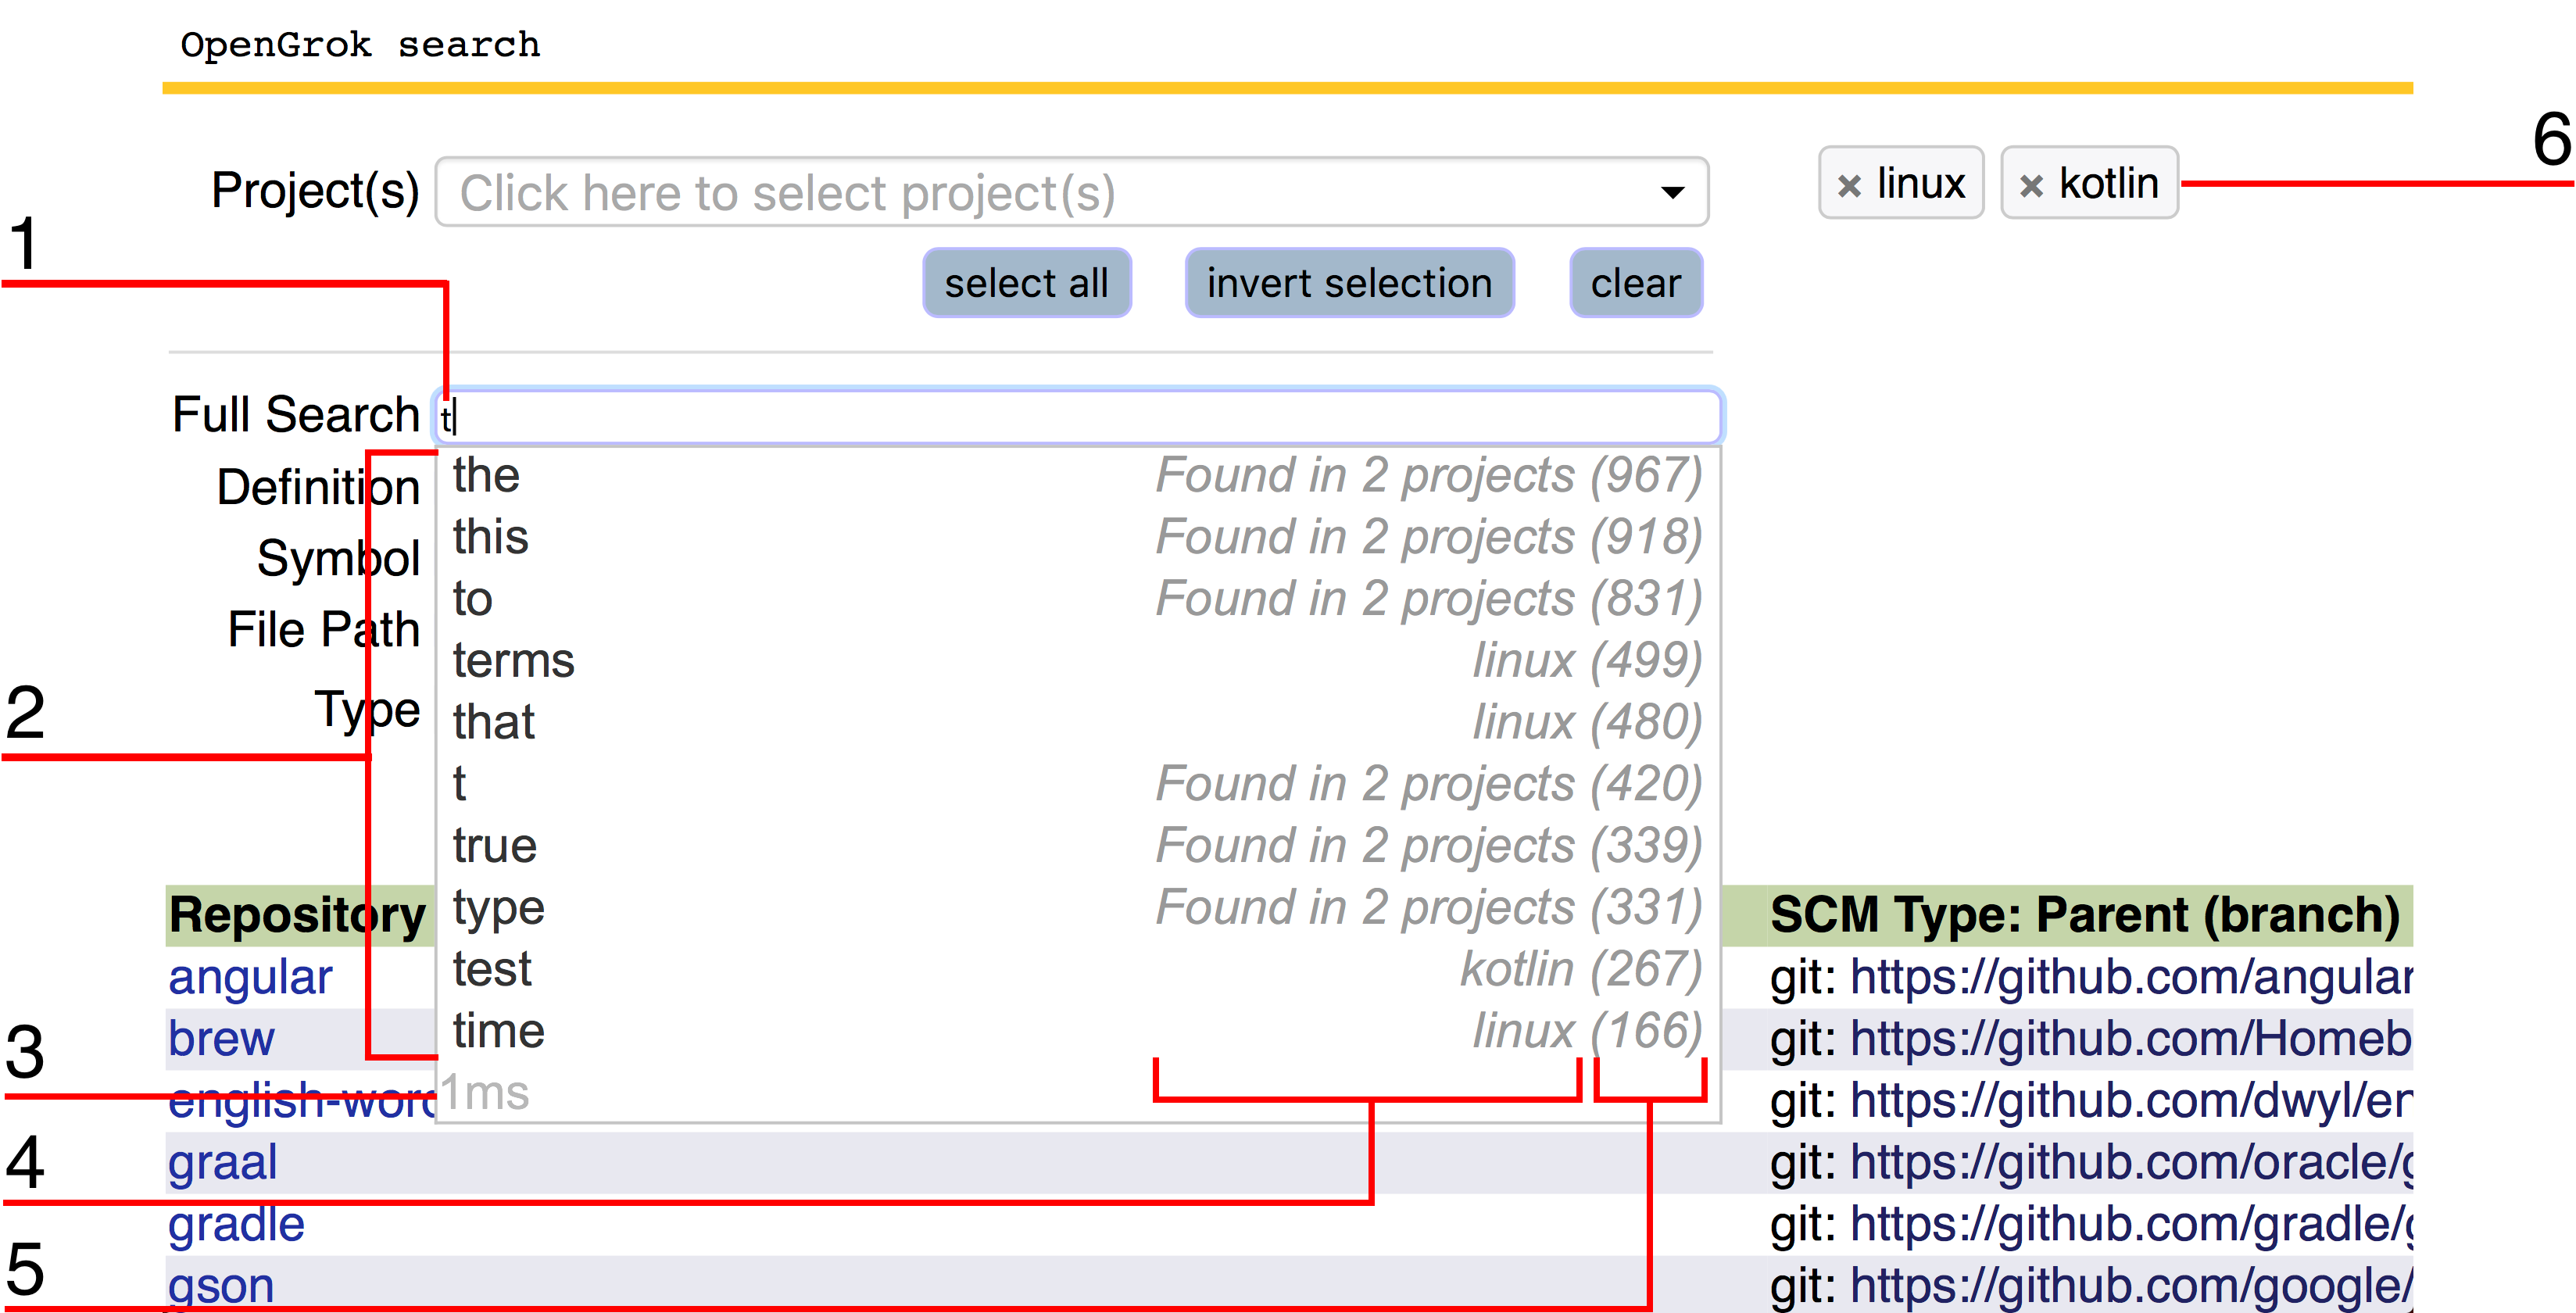
\includegraphics[width=145mm]{../img/suggestions_pic.png}
    \caption{Suggestions example}
    \label{suggestions_pic}
\end{figure}

The numbers in the Figure \ref{suggestions_pic} represent:
\begin{enumerate}
    \item Typed value into the search field. In this case letter \textit{t}.
    \item List of suggestions.
    \item Time it took to generate the suggestions. (Optional.)
    \item In which projects the term was found. (Optional.)
    \item Score of the terms. (Optional.)
    \item Projects for which suggestions are shown.
\end{enumerate}

\subsection{Selecting the Suggestions}
The suggestions can be navigated by using:
\begin {itemize}
    \item \textbf{Keyboard} – the suggestion can be focused by using up $\uparrow$ and down $\downarrow$ arrow keys.
    The suggestion can be selected by pressing the \textit{enter} (carriage return) or \textit{tab} key.
    The suggestions window can also be closed by pressing the \textit{esc} key.
    \item \textbf{Mouse} – by hovering over the suggestion it is focused. By clicking on the suggestion it
    is selected.
\end{itemize}

\subsubsection{Focused Suggestion}
If a suggestion is focused, then its background color is changed to \textit{blue}. In case of keyboard focus,
the text of the field shows the result value as if this suggestion was selected.
It looks like in the Figure \ref{suggestion_focused}.

\begin{figure}[htbp]
    \centering
    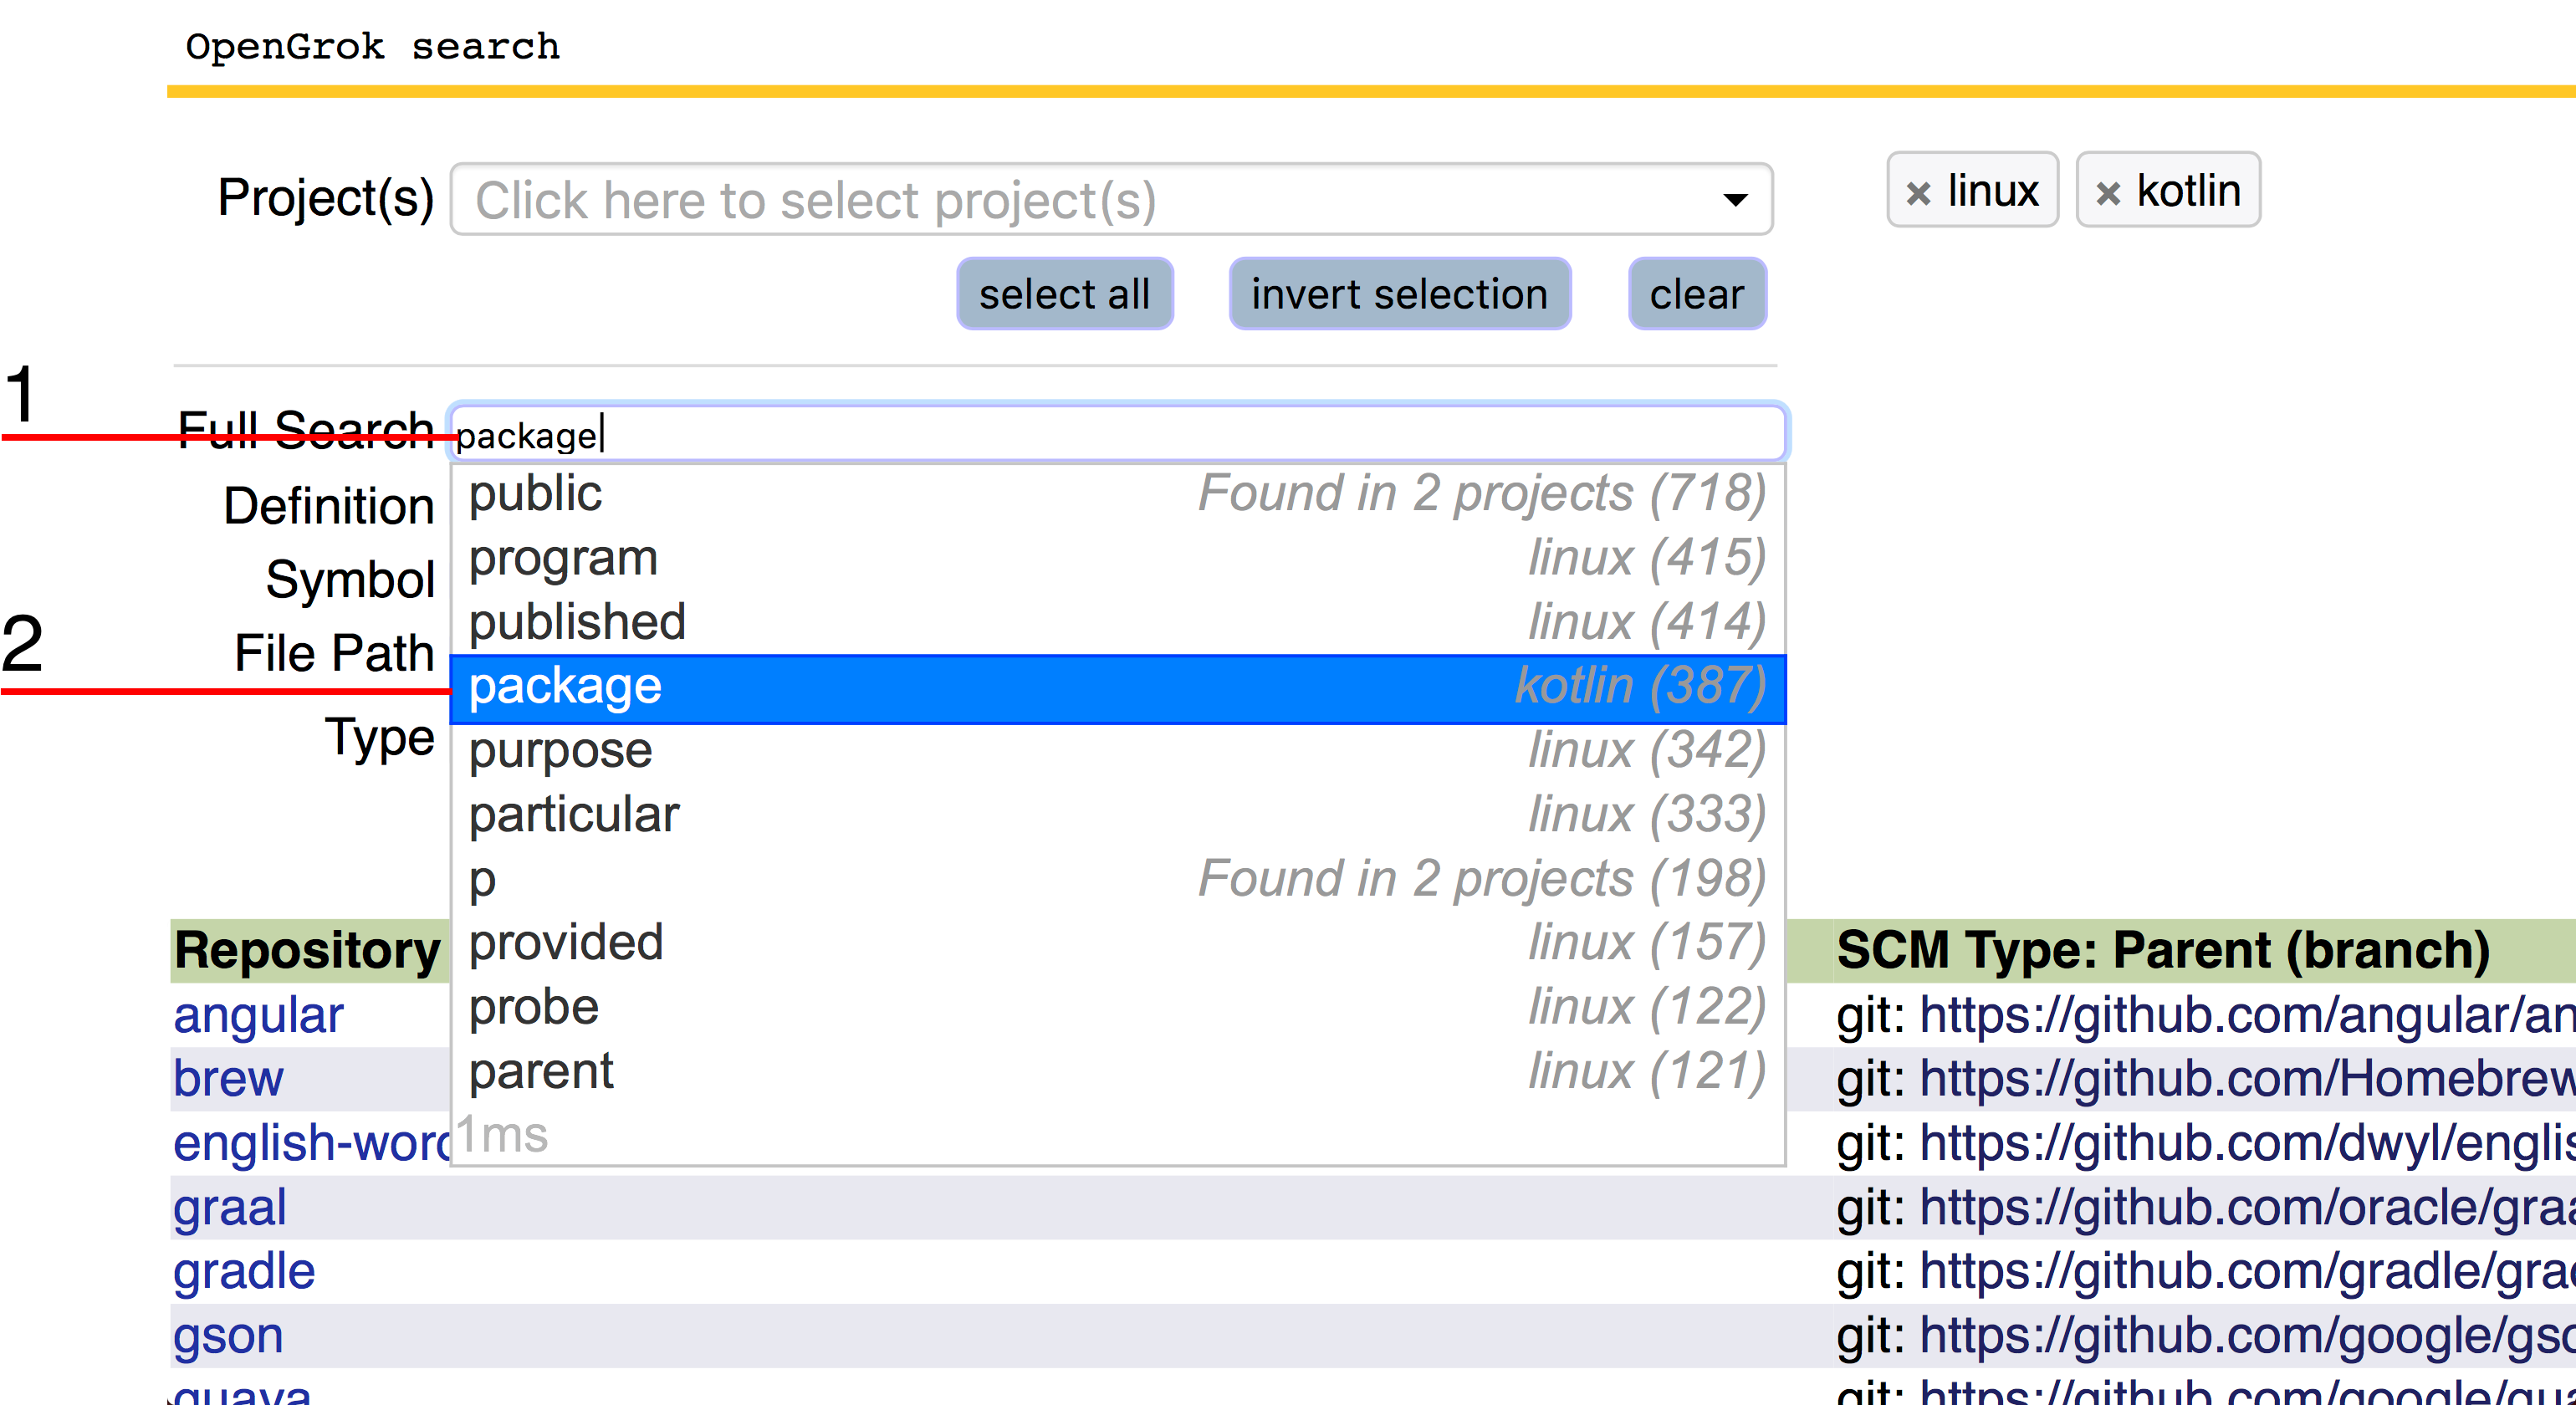
\includegraphics[width=145mm]{../img/suggestions_focused.png}
    \caption{Focused suggestion}
    \label{suggestion_focused}
\end{figure}

The numbers in the Figure \ref{suggestion_focused} represent:
\begin{enumerate}
    \item The field already contains the value \textit{package} even though only the prefix \textit{p} is actually written.
    \item Focused suggestion.
\end{enumerate}

\subsubsection{Errors}
It might be a common occurrence that users type an invalid query. For instance, \textit{)} is missing at the end of
the query \textit{(test}. Therefore, the user is notified if the Lucene cannot parse the query or some other
error occurs. This case is pictured in the Figure \ref{suggestions_error}.

\begin{figure}[htbp]
    \centering
    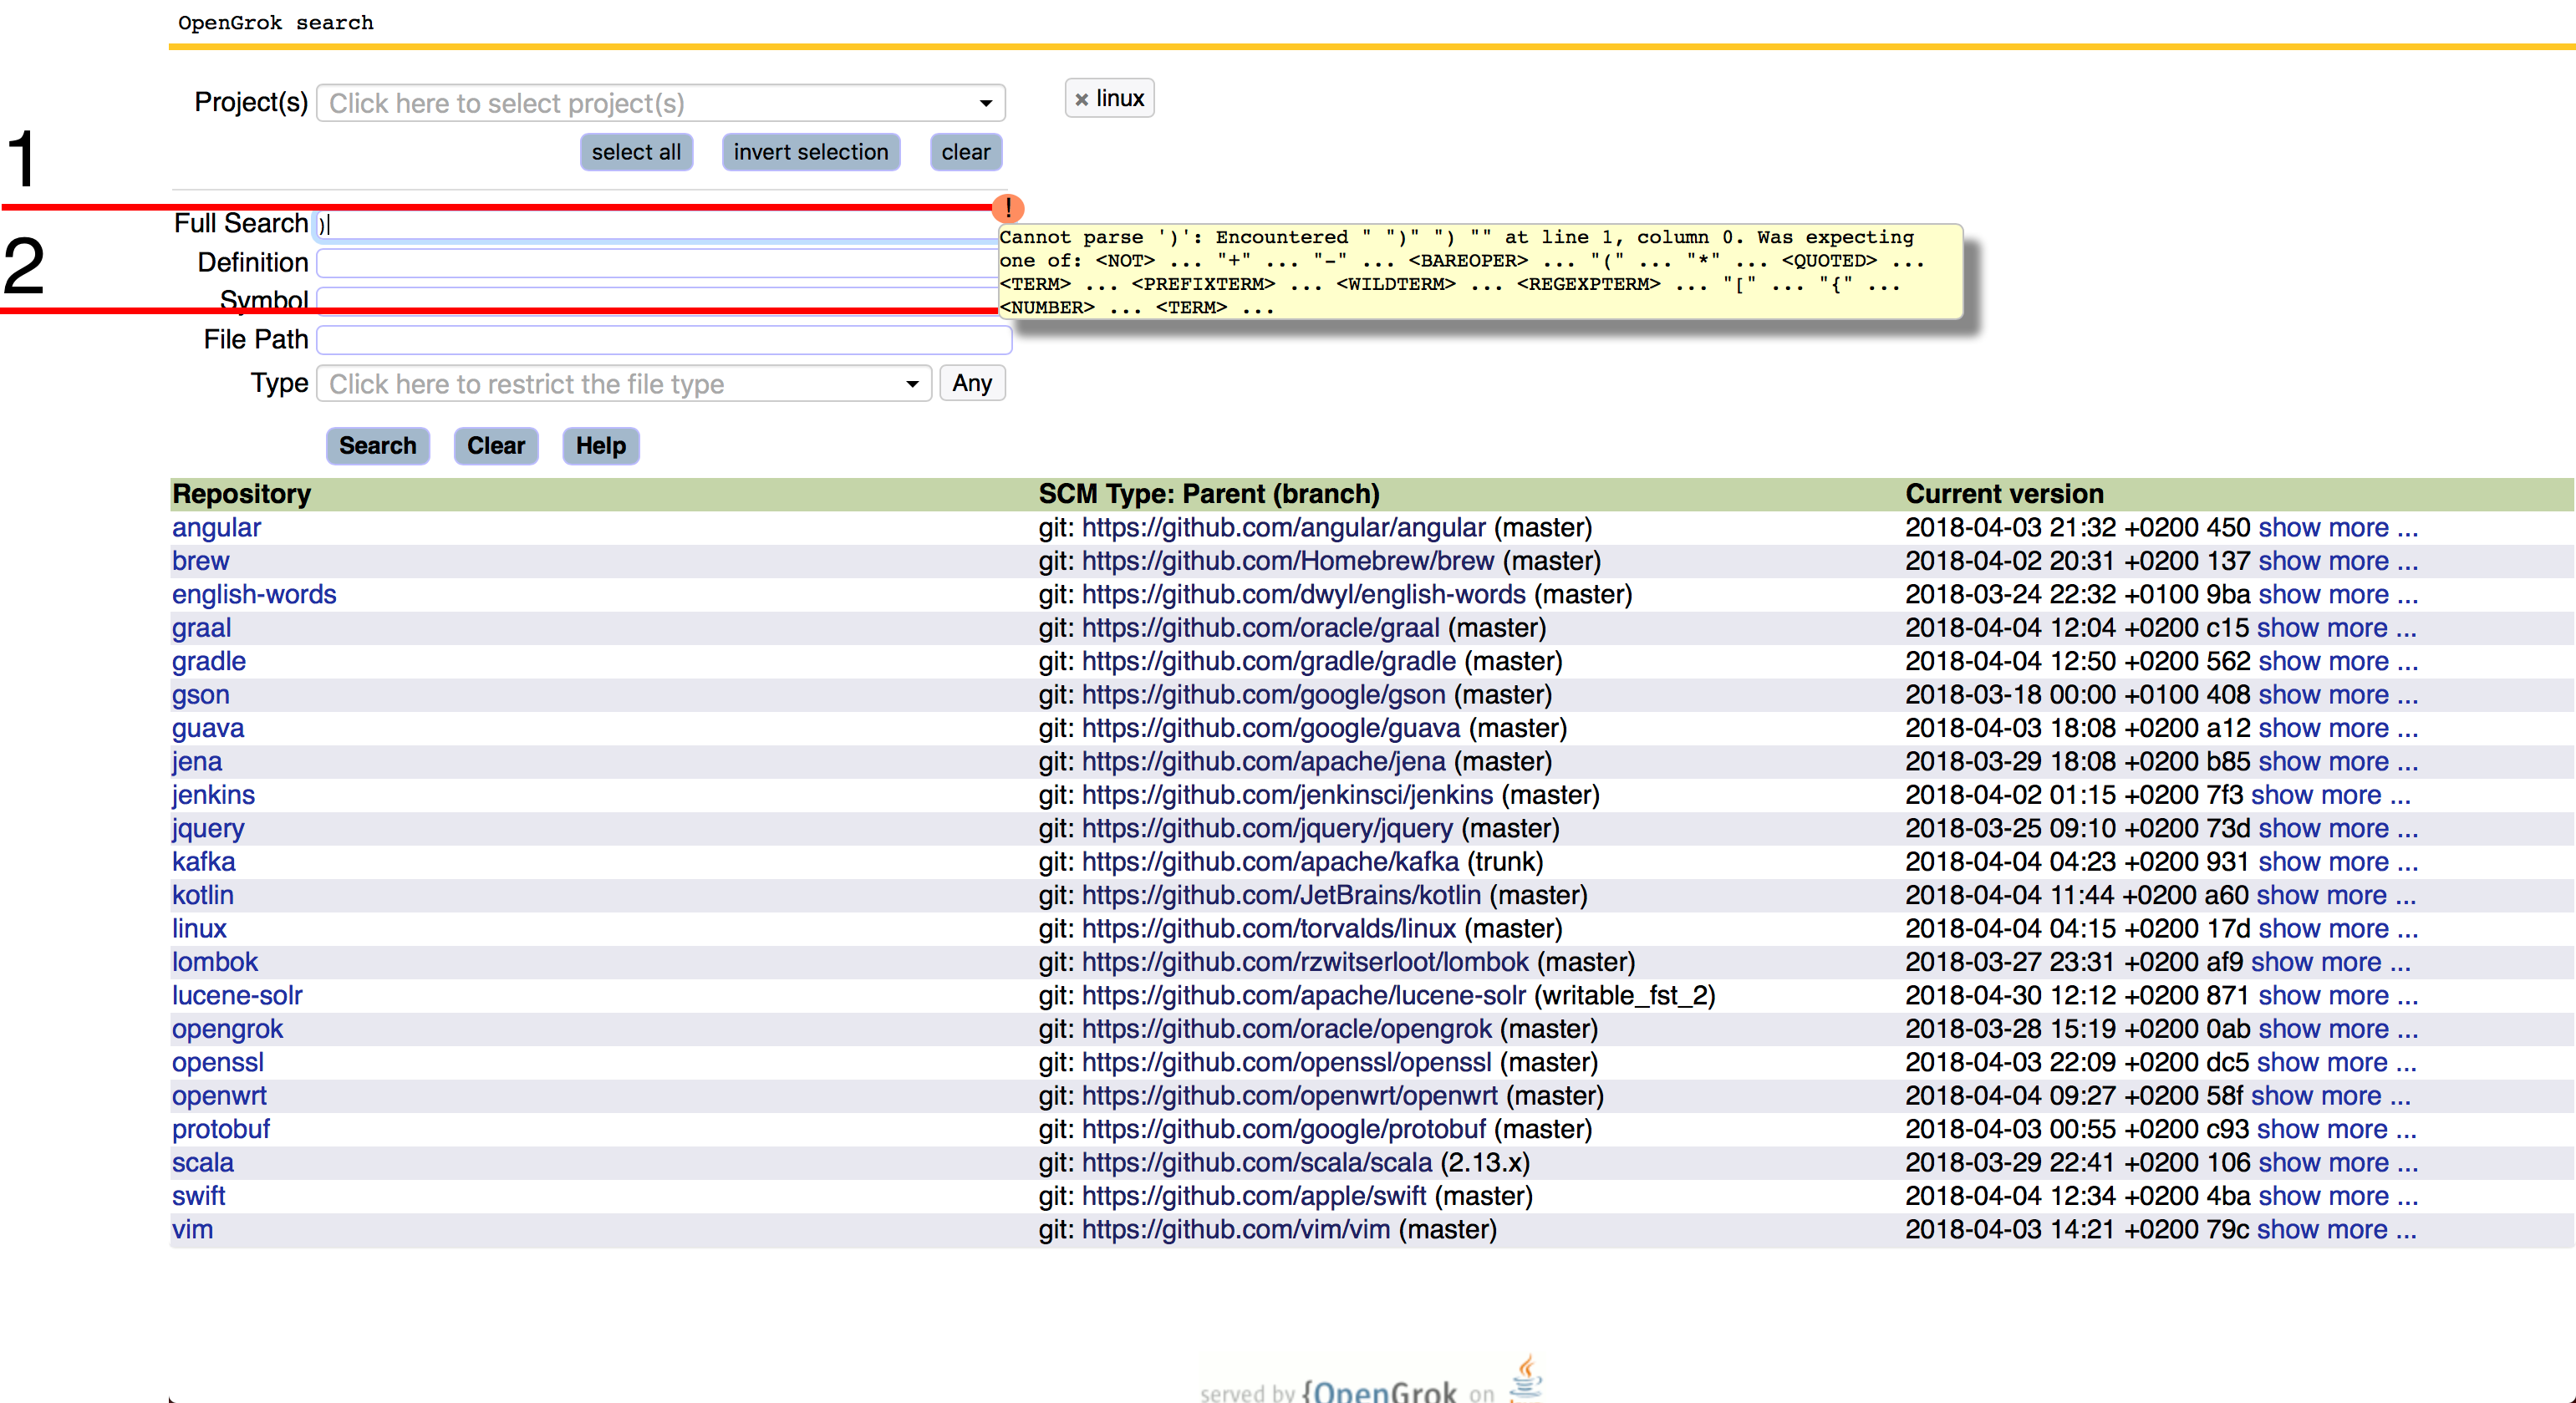
\includegraphics[width=145mm]{../img/suggestions_error.png}
    \caption{Suggestions error}
    \label{suggestions_error}
\end{figure}

The numbers in the Figure \ref{suggestions_error} represent:
\begin{enumerate}
    \item Error notification.
    \item Detail of the error. This is only shown if the user hovers over the error notification.
\end{enumerate}

\subsubsection{Minisearch}
While traversing a source code or history, a minisearch field is available in the navigation menu. It allows users
to search in the current project. The suggestions are enabled for it as well. The result can look like in the Figure
\ref{suggestions_minisearch}.

\begin{figure}[htbp]
    \centering
    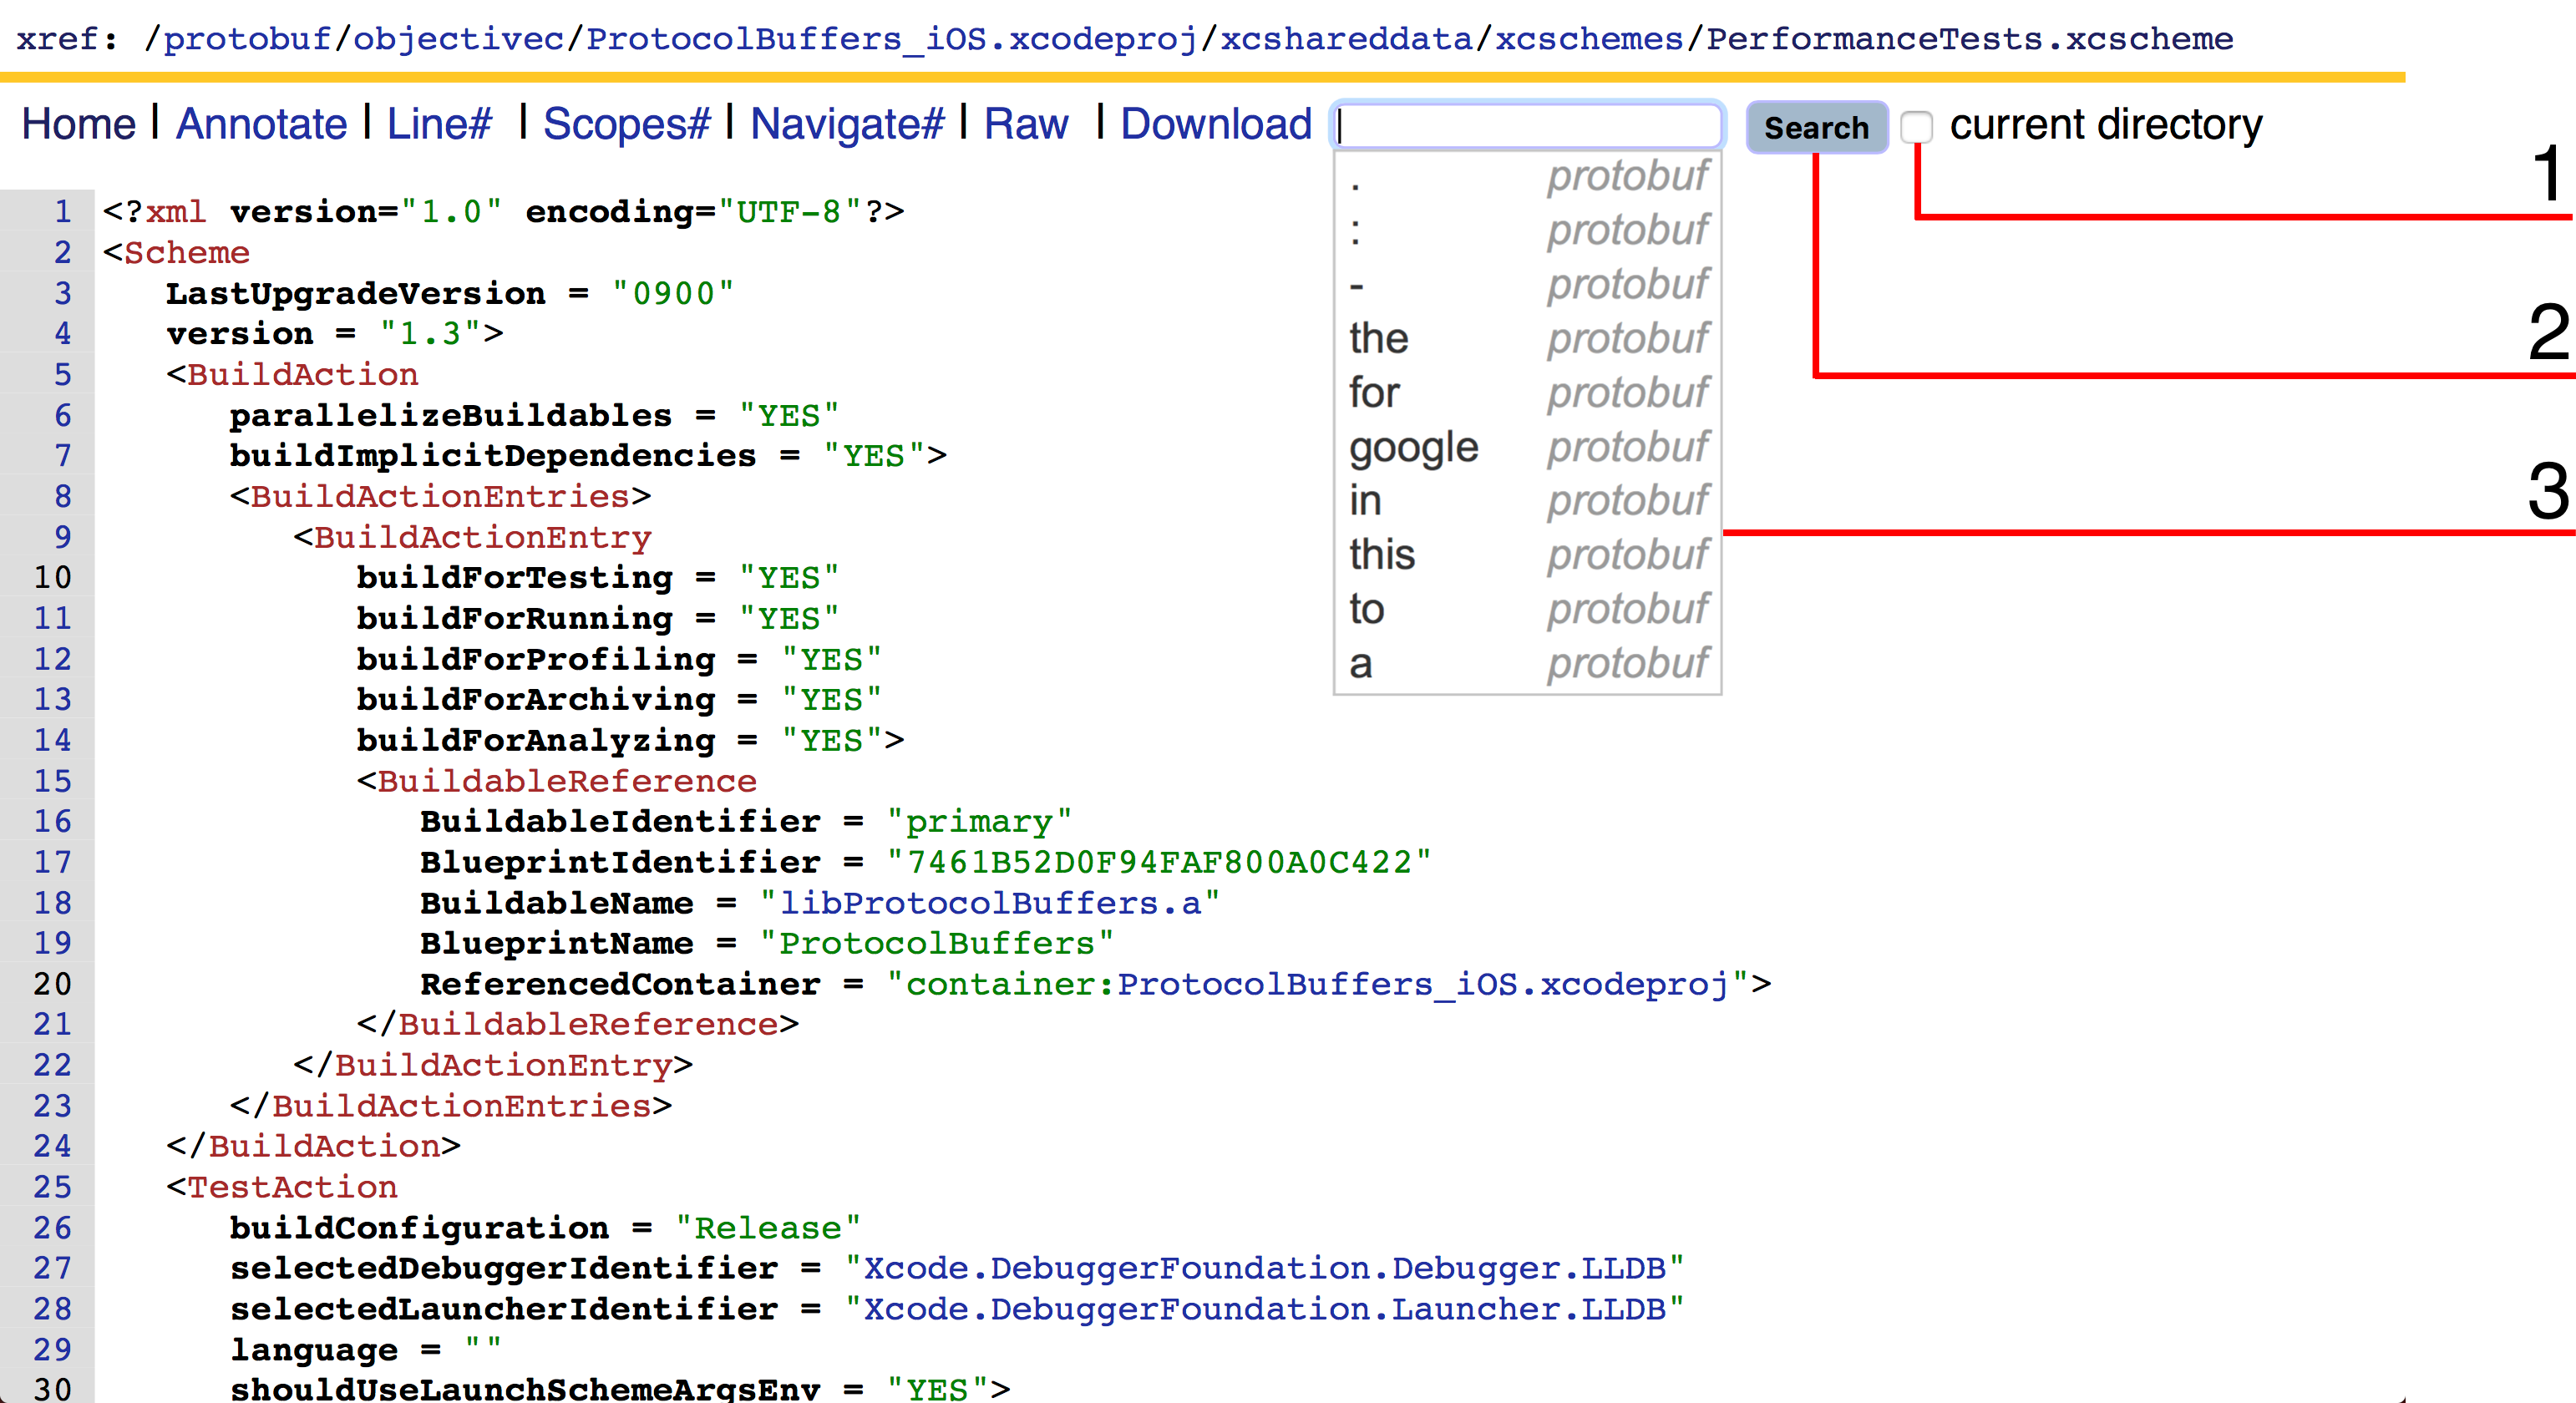
\includegraphics[width=145mm]{../img/minisearch.png}
    \caption{Suggestions for minisearch}
    \label{suggestions_minisearch}
\end{figure}

In the Figure \ref{suggestions_minisearch} the numbers represent:
\begin{enumerate}
    \item Checkbox that specifies if the search (and consequently suggestions) should be restricted to the directory
    in which the displayed file is located. In this example it adds the following value to the \textit{path} field:
\begin{code}
"/protobuf/objectivec/ProtocolBuffers_iOS.xcodeproj/xcshareddata/
xcschemes/"
\end{code}
    \item Search button that launches the search.
    \item Suggestions window as described before.
\end{enumerate}

\subsubsection{Timeout}
As specified in \ref{restricting_load}, the system may be under load and it might return only a partial result or no
suggestions at all. In the case of the partial result, the message \textit{"Partial result due to timeout"} will be
displayed at the bottom of the suggestions window similarly as in the Figure \ref{partial_result}.
\begin{figure}[htbp]
    \centering
    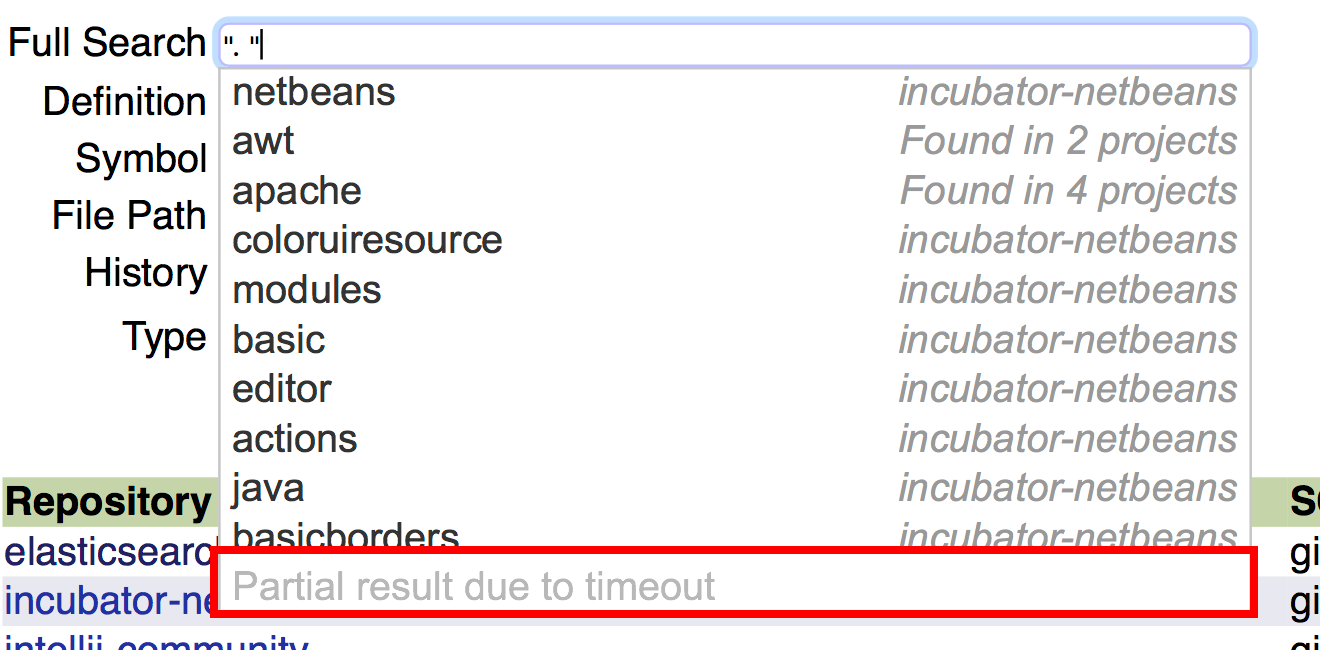
\includegraphics[width=100mm]{../img/partial_result.png}
    \caption{Message if only partial result was returned}
    \label{partial_result}
\end{figure}

If no suggestions were returned, then
it may signify two cases:
\begin{itemize}
    \item The query yields no results. In that case a message \textit{"No matches found"} will be displayed as in the
    Figure \ref{no_matches}.
    \begin{figure}[htbp]
        \centering
        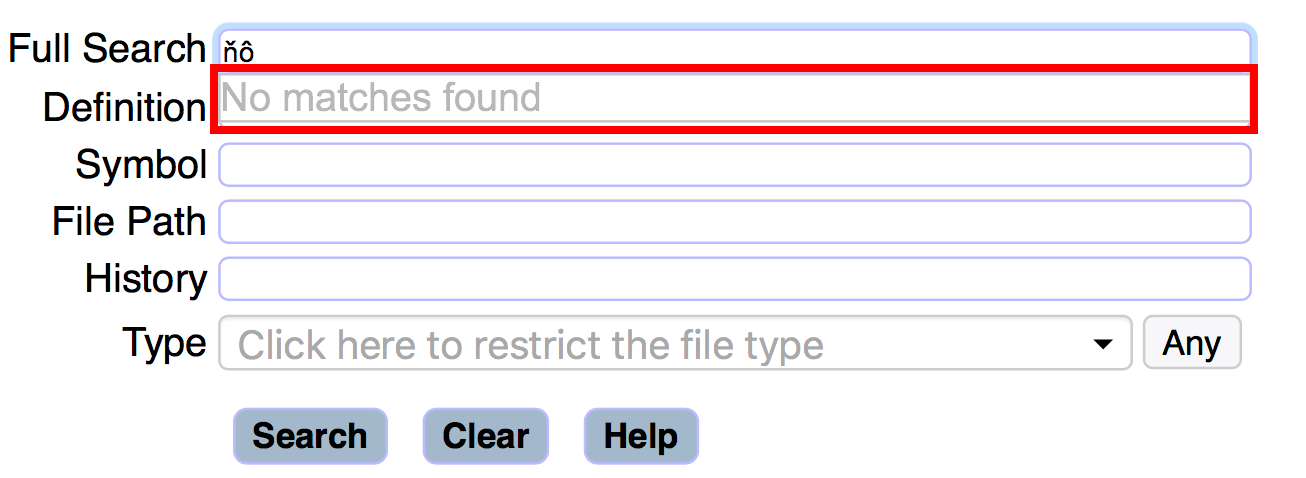
\includegraphics[width=100mm]{../img/no_matches.png}
        \caption{Message if no matches were found for the specified query}
        \label{no_matches}
    \end{figure}

    \item The system timed out and did not find any possible suggestions. In that case no suggestions window will be displayed.
\end{itemize}

\section{Administrator Guide}
\label{administrator_guide}

There are multiple ways to modify the suggester configuration described in \ref{suggester_config}:
\begin{itemize}
    \item By modifying the OpenGrok's XML configuration described in \ref{opengrok_configuration}. An example:
\begin{code}
<java version="1.8.0_162" class="java.beans.XMLDecoder">
  <object
      class="org.opensolaris.opengrok.configuration.Configuration"
      id="Configuration0">
    <void property="suggesterConfig">
      <void property="allowComplexQueries">
        <boolean>false</boolean>
      </void>
      <void property="allowMostPopular">
        <boolean>false</boolean>
      </void>
      <void property="allowedFields">
        <object class="java.util.Collections" method="singleton">
          <string>defs</string>
        </object>
      </void>
      <void property="allowedProjects">
        <object class="java.util.Collections" method="singleton">
          <string>fruitonserver</string>
        </object>
      </void>
      <void property="enabled">
        <boolean>false</boolean>
      </void>
      <void property="maxProjects">
        <int>2</int>
      </void>
      <void property="maxResults">
        <int>11</int>
      </void>
      <void property="minChars">
        <int>2</int>
      </void>
      <void property="rebuildCronConfig">
        <string>5 * * * *</string>
      </void>
      <void property="showProjects">
        <boolean>false</boolean>
      </void>
      <void property="showScores">
        <boolean>true</boolean>
      </void>
      <void property="showTime">
        <boolean>true</boolean>
      </void>
      <void property="buildTerminationTime">
        <int>500</int>
      </void>
    </void>
  </object>
</java>
\end{code}
    \item By using the REST API configuration endpoint. It is possible to send a JSON representation of the suggester
    configuration. Only the properties which differ from the default configuration need to be specified. Example data:
\begin{code}
{"enabled": "false"}
\end{code}
    Suggester configuration endpoint:
\begin{code}
/api/v1/configuration/suggesterConfig
\end{code}

\end{itemize}

\chapter{Program Documentation}
\label{chap:program}

This chapter focuses on the implementation part of the thesis.

\section{Overview}
As mentioned, suggestions are retrieved by a REST API call made to the Web module. This module processes the data and
invokes the Suggester module to return the suggestions. Simplified diagram which shows the main interactions between the
objects and modules can be seen in the Figure \ref{programmer_sequence}.
\begin{figure}[htbp]
    \centering
    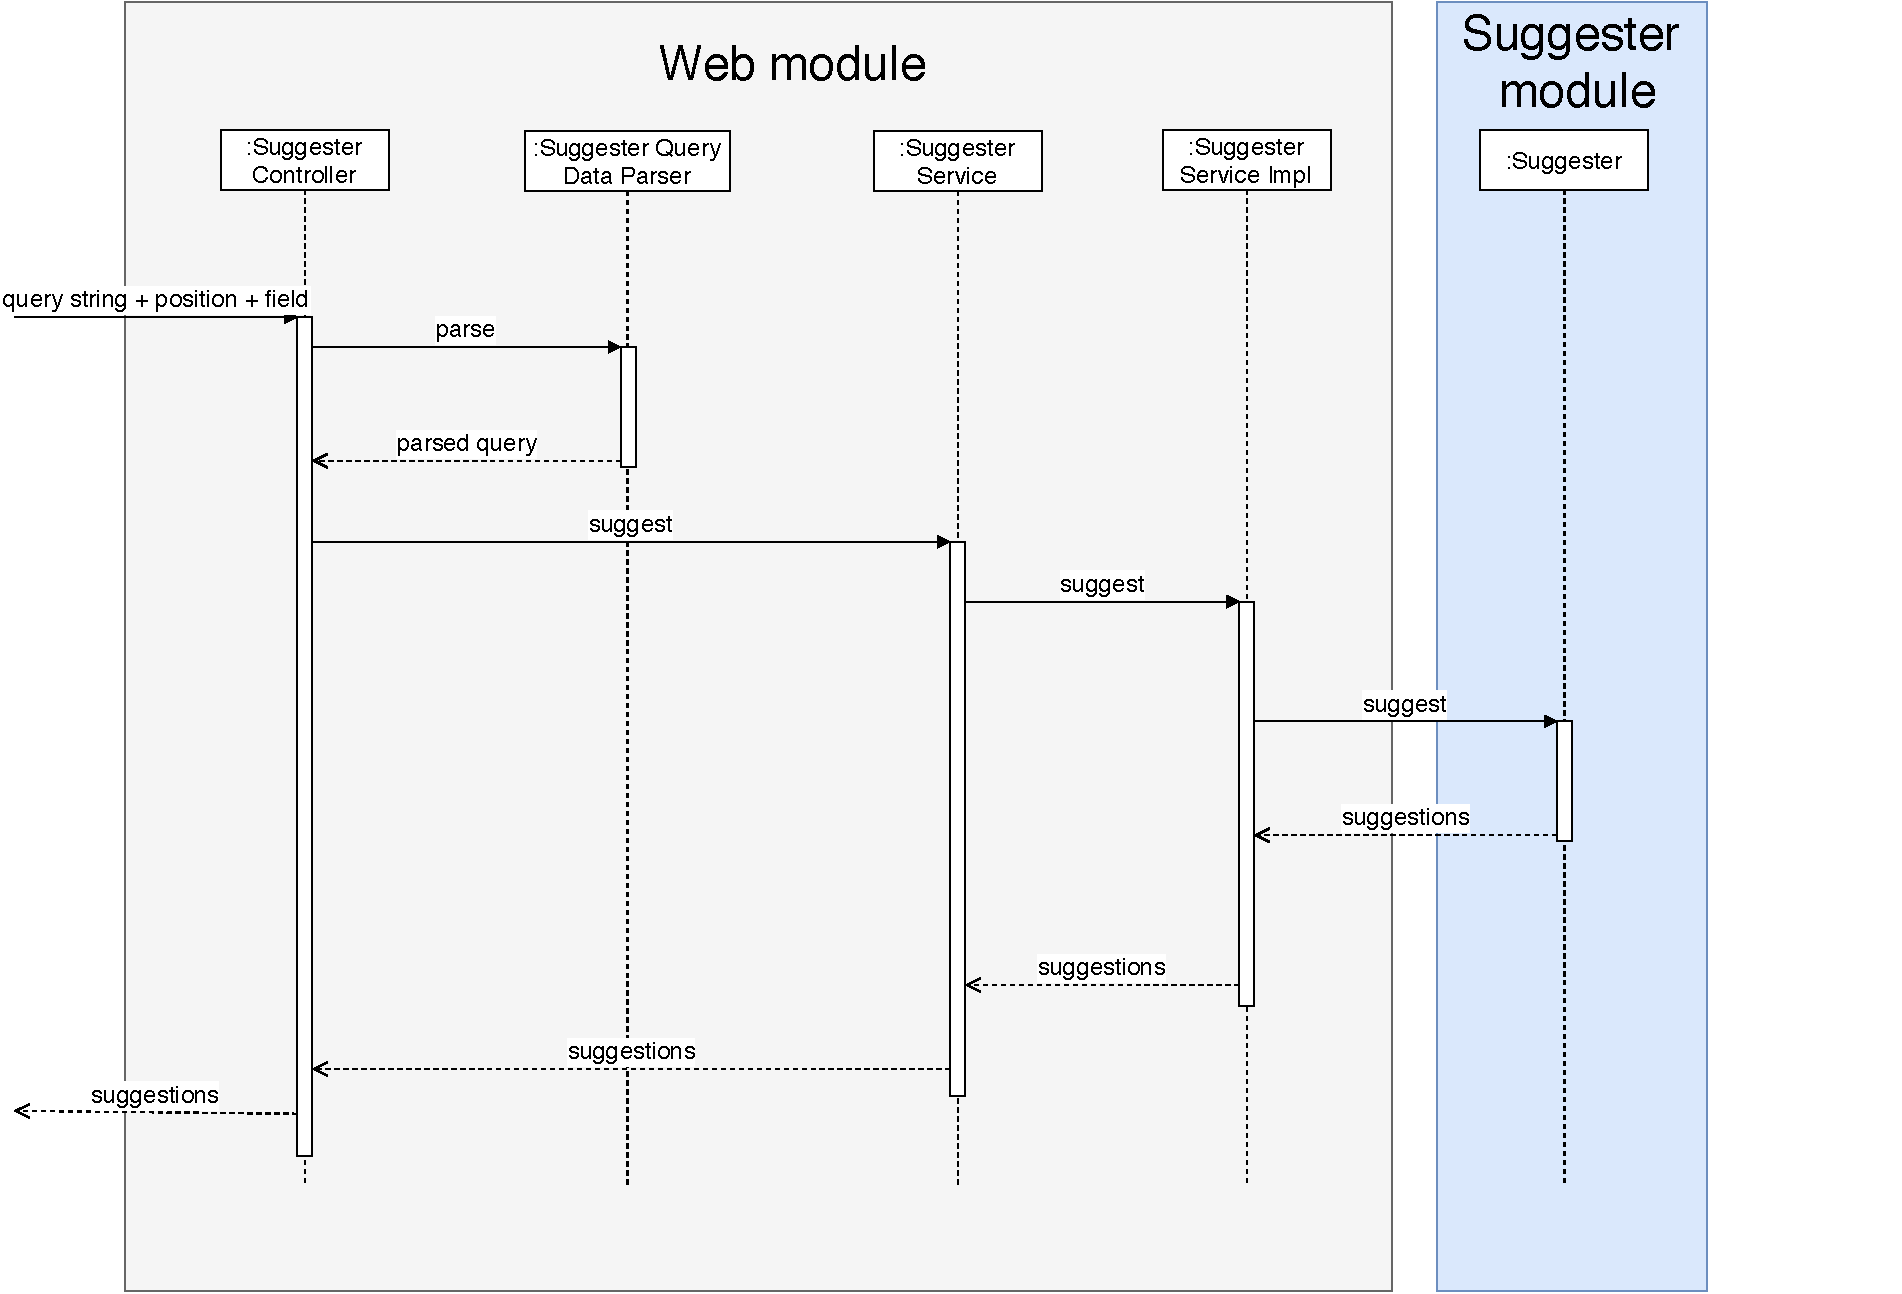
\includegraphics[width=145mm]{../img/programmer_sequence.pdf}
    \caption{Overview of the main object interactions}
    \label{programmer_sequence}
\end{figure}

\section{Web module}
The suggester support was added as a part to the already existing OpenGrok's REST API. The \textit{SuggesterController}
class serves as a REST API endpoint for suggester related queries. Other needed classes are located in the
\textit{org.opensolaris.opengrok.web.api.v1.suggester} package. Classes which are auto-detected by the Jersey
implementation are located in the \textit{org.opensolaris.opengrok.web.api.v1.suggester.provider} package and are annotated
by the \textit{@Provider}\footnote{\url{https://docs.oracle.com/javaee/7/api/javax/ws/rs/ext/Provider.html}} annotation.
The communication with the Suggester module is abstracted in the \textit{SuggesterService} interface and implemented in the
\textit{SuggesterServiceImpl} class. The implementation is injected into the classes which require the
\textit{SuggesterService} by the use of
\textit{@Inject}\footnote{\url{https://docs.oracle.com/javaee/7/api/javax/inject/Inject.html}} annotation. If some other
component which is not part of the REST API part of the application needs to access the \textit{SuggesterService},
it can retrieve it by invoking \textit{getDefault()} method in the \textit{SuggesterServiceFactory} class.

\subsubsection{Configuration Change}
The suggester data structures need to be refreshed on configuration change.
Many basic OpenGrok properties might have changed, for instance:
\begin{itemize}
    \item \textit{dataRoot} which specifies where OpenGrok stores the data.
    \item Suggester configuration.
    \item Projects.
\end{itemize}

It is not trivial to notice all the changes and it would not be feasible from the modifiability point of view to check
specific values for change. Therefore, \textit{SuggesterServiceImpl} closes the underlying suggester data structures
and tries to reinitialize the suggester with the new configuration. If the configuration has not changed in a major
aspect (e.g. different \textit{dataRoot} or new projects were added), then the Suggester module just reloads the data
from disk. Reload from disk should be fast (from the experience less than $1$ s).

\section{Suggester module}
The Suggester module is located under the \textit{suggester} directory of the root of the project. The main class which
exposes the suggester functionality is the \textit{Suggester} class.

\subsubsection{Public API}
\label{public_api}
The public API consists of the following methods:
\begin{itemize}
    \item \textit{init(Collection\textless NamedIndexDir\textgreater)} – initializes all the data structures based on the paths
    to the indexes and their names (project names).
    \item \textit{remove(Iterable\textless String\textgreater)} – removes all the data structures stored for the
    specified names.
    \item \textit{search(List\textless NamedIndexReader\textgreater, SuggesterQuery, Query)} –
    searches the suggester data and returns suggestions to the provided queries.
    \item \textit{onSearch(Iterable\textless String\textgreater, Query)} –
    event signalization that the query was searched. Updates the data structures for the most popular completion.
    \item \textit{increaseSearchCount(String, Term, int)} – updates the search count for the specified project and term by the
    specified int value. Negative values are not allowed.
    \item \textit{getSearchCounts(String, String, int, int)} – returns popularity data for the specified project and field.
    \item \textit{close()} – closes the suggester data structures and other functionality.
\end{itemize}

\subsubsection{Suggester Data}
The following shows the typical \textit{dataRoot} content for a multi-project OpenGrok setup along with the suggester data.
\dirtree{%
.1 \textit{dataRoot}\DTcomment{OpenGrok's data root specified in the configuration}.
.2 historycache\DTcomment{history data for files}.
.3 project1\DTcomment{history data for files of \textit{project1}}.
.4 {…}.
.3 {…}.
.2 index\DTcomment{index data}.
.3 project1\DTcomment{index data for \textit{project1}}.
.4 {…}.
.3 {…}.
.2 statistics.json\DTcomment{stored statistics data}.
.2 suggester\DTcomment{suggester data}.
.3 project1\DTcomment{suggester data for \textit{project1}}.
.4 \{field\}\_map.cfg\DTcomment{stored Chronicle Map configuration}.
.4 \{field\}\_search\_count.db\DTcomment{stored Chronicle Map}.
.4 \{field\}.wfst\DTcomment{stored WFST data structure}.
.4 version.txt\DTcomment{version of the suggester data}.
.3 {…}.
.2 timestamp\DTcomment{timestamp of last indexing}.
.2 xref\DTcomment{pre-generated HTML files}.
.3 project1\DTcomment{pre-generated HTML files for \textit{project1}}.
.4 {…}.
.3 {…}.
}

In the case of a single-project OpenGrok setup, there is no \textit{project1} as specified in the previous example but the
data are stored directly in directories \textit{historycache, index, suggester} and \textit{xref}.

The \textit{\{field\}} represents the Lucene field for which the files contain the data, e.g. \textit{full}.
If some data are corrupted and
the suggester is not able to read them, the best solution might be:
\begin{enumerate}
    \item If possible, then backup the popularity data as specified in \ref{retrieving_popularity_data}. (Not needed
    if popularity data is not important or turned off.)
    \item Stop the web application.
    \item Remove either the corrupted data or the whole suggester directory.
    \item Start the web application again.
    \item Initialize the popularity data as specified in \ref{increasing_search_counts}. Some data modifications would
    be needed; however, if the need arises, an automatic tool might be created for this purpose. (Not needed
    if popularity data is not important or turned off.)
\end{enumerate}

\subsubsection{Detecting Index Version}
The Indexer might run even if the Web application is turned off. Therefore, it would not be possible to notify the
Suggester about the change. As a result, the Suggester needs to detect this by itself. Exactly for this purpose serves the
aforementioned file \textit{version.txt}. It contains a number which specifies the generation of the last index commit
for which the data were created.
Upon detecting that the data version does not match with the index version, the suggester will rebuild its data by itself.

\subsubsection{Data Structures Abstractions}
The implementation contains interfaces for data structures so the implementation might change and there would be no need to
modify other parts of the Suggester module. Abstract data structures:
\begin{itemize}
    \item \textbf{PopularityMap} - abstraction for most popular completion.
    \item \textbf{IntsHolder} – abstraction for holding a set of positions in a document used for Phrase Query evaluation.
\end{itemize}

\section{Testing}
Unit tests\footnote{\url{https://en.wikipedia.org/wiki/Unit_testing}} were written for the Suggester module to test
the basic functionality. They can be found in a standard Maven test directory \textit{src/test/java}.

To test the real word usage and to test the integration with other OpenGrok modules,
tests were written for \textit{SuggesterController} which test the
suggester endpoint in the Web module which in turn calls various parts from Indexer and Suggester modules.
Small projects written in variety of programming languages used for OpenGrok's own testing were used as the test data.
These can be found in the \textit{testdata/sources} directory of the OpenGrok project root.
First of all, these projects are copied into the temporary \textit{sourceRoot} directory. Then they are indexed.
After that, the Suggester is initialized. Finally, the tests run.

However, the tests are not exhaustive and for better test coverage more tests should be written.

Regarding UI testing, OpenGrok does not have any UI tests in place. Therefore, it was not deemed to be a high priority.
In the future, it would make sense to incorporate at least some UI testing.
\chapter{Impact on the OpenGrok project}
\label{chap:impact}

\textit{Change impact analysis}\footnote{\url{https://en.wikipedia.org/wiki/Change\_impact\_analysis}} is a field of
study which task is to determine what impact the changes may have on the system. Sometimes, it is very hard to analyze
the impact of a change. Even more so in a large projects with a huge codebase. Analysis of the main decisions made is
described in detail in the chapter \ref{chap:analysis}. The main aspects of the added changes that can be discussed are:
\begin{itemize}
    \item Impact on the search results. Discussed in more detail in \ref{search_res_impact}.
    \item Impact on the hardware requirements. Discussed in more detail in \ref{hw_req_impact}.
\end{itemize}

\section{Impact on the Search Results}
\label{search_res_impact}
It is hard to compare search results; therefore, search engines as well. Which search engine performs better, the one
that returns only a few relevant documents but omitted many in the process or the one that returns all relevant
documents but includes some that are not?
In information retrieval field there are measurements which take this into account, most notable are \textbf{precision}
and \textbf{recall}\footnote{\url{https://en.wikipedia.org/wiki/Precision\_and\_recall}}.

\textbf{Precision} is the fraction of retrieved documents that are relevant to the query. Equation can be seen on
\ref{precision_eq}.

\begin{equation}
\label{precision_eq}
precision = \frac{\vert \{relevant\ documents\} \cap \{ retrieved\ documents \} \vert}{\vert \{ retrieved\ documents \} \vert}
\end{equation}

\textbf{Recall} is the fraction of the relevant documents that are successfully retrieved. Equation can be seen on
\ref{recall_eq}.

\begin{equation}
\label{recall_eq}
recall = \frac{\vert \{relevant\ documents\} \cap \{ retrieved\ documents \} \vert}{\vert \{ relevant\ documents \} \vert}
\end{equation}

However, suggester does not impact these measurements directly. The same query returns the same results with or without
the suggester. Nevertheless, suggester affects them indirectly:
\begin{itemize}
    \item There are less queries which yield no results – if the user types a few characters and there are no suggestions then he
    can immediately see that there are no terms with that prefix. Therefore, the result will be empty.
    \item Probably negative impact on precision because of the scoring described in \ref{prefix_scoring}. The terms which
    are in more documents have greater scores. Thus, these terms are promoted and are more likely to be chosen by the user.
    Therefore, the size of retrieved documents set will be greater. However, the initial scoring might be mitigated
    by taking into account previous users' searches as described in \ref{previous_searches}.
\end{itemize}

It is not easy to achieve feasible values for both precision and recall. In many information retrieval systems when one is
being increased the other one decreases. This is most notable in Boolean Information Retrieval Model
\footnote{\url{https://en.wikipedia.org/wiki/Standard\_Boolean\_model}}.

\section{Impact on the hardware requirements}
\label{hw_req_impact}
The most affected resources are:
\begin{itemize}
    \item \textbf{CPU} – in simple situations where only a prefix is typed the CPU load is not that high because it
    is a lookup in WFST data structure which is optimized for this kind of scenarios. However, in other cases
    index searches are performed which can consume a lot of CPU resources.
    \item \textbf{Memory} – WFST data structures are held in memory. Although their memory footprint is very low,
    one data structure needs to be created per Lucene field per project which can sum up to a signifcant value.
    Also, data for most popular completion are stored in the Chronicle Map implementation which provide additional
    memory consumption.
    \item \textbf{Disk} – the WFST data structure are stored on the disk to provide a quick startup.
    Data for most popular completion need to be stored as well.
\end{itemize}

\section{Impact on the demo instance}
For monitoring the impact of the suggester, a demo instance was created which can be accessed on the url
\url{http://demo.opengrok.org}. This instance contains 5 projects:
\begin{itemize}
    \item \textbf{elasticsearch}\footnote{\url{https://github.com/elastic/elasticsearch}} – scalable search engine built
    upon Apache Lucene.
    \item \textbf{NetBeans}\footnote{\url{https://github.com/apache/incubator-netbeans}} – NetBeans IDE in development
    under ASF\footnote{\url{https://en.wikipedia.org/wiki/Apache\_Software\_Foundation}}.
    \item \textbf{IntelliJ IDEA Community Edition}\footnote{\url{https://github.com/JetBrains/intellij-community}} –
    open-source edition of the popular IDE.
    \item \textbf{Lucene/Solr}\footnote{\url{https://github.com/apache/lucene-solr}} – combined repository for Apache
    Lucene and Apache Solr.
    \item \textbf{OpenGrok}
\end{itemize}
However, real instances may and often do contain more projects.

The demo instance uses Apache Tomcat servlet container. Many solutions exist which provide a possibility to monitor
applications in a Tomcat instance. From those the most significant are:
\begin{itemize}
    \item \textbf{JMX\footnote{\url{https://en.wikipedia.org/wiki/Java\_Management\_Extensions}} remote} –
    Tomcat provides possiblity to manage and monitor the applications via JMX. Many applications use this functionality
    to their advantage.
    \item \textbf{JavaMelody}\footnote{\url{https://github.com/javamelody/javamelody}} – can be added to the project as a
    dependency and creates a simple page with monitoring information available at \textit{application\_URI/monitoring}.
    Provides monitoring of CPU, memory usage, HTTP requests count and many others. Also allows exporting data in
    various formats, e.g. PDF, JSON. The main disadvantage is that it is embedded into the application and may influence
    the gathered data. However, this overhead is small, e.g. the memory overhead did not exceed 3MiB.
    \item \textbf{PSI Probe}\footnote{\url{https://github.com/javamelody/javamelody}} – deployed as a separate
    application into the Apache Tomcat instance. Uses JMX exported by Tomcat. The disadvantages are:
    \begin{itemize}
        \item Cannot export data in common exchange formats. However, raw XML data are created under the Tomcat
        home directory.
        \item Data are not persistent.
    \end{itemize}
\end{itemize}

\textbf{Chosen solution} JavaMelody was chosen because of its simplicity and because it provided all the needed
features despite the small overhead.


\chapter*{Conclusion}
\addcontentsline{toc}{chapter}{Conclusion}


%%% Bibliography
%%% Bibliography (literature used as a source)
%%%
%%% We employ bibTeX to construct the bibliography. It processes
%%% citations in the text (e.g., the \cite{...} macro) and looks up
%%% relevant entries in the bibliography.bib file.
%%%
%%% The \bibliographystyle command selects, which style will be used
%%% for references from the text. The argument in curly brackets is
%%% the name of the corresponding style file (*.bst). Both styles
%%% mentioned in this template are included in LaTeX distributions.

\bibliographystyle{plainnat}    %% Author (year)
% \bibliographystyle{unsrt}     %% [number]

\renewcommand{\bibname}{Bibliography}

%%% Generate the bibliography. Beware that if you cited no works,
%%% the empty list will be omitted completely.

\bibliography{bibliography}

%%% If case you prefer to write the bibliography manually (without bibTeX),
%%% you can use the following. Please follow the ISO 690 standard and
%%% citation conventions of your field of research.

% \begin{thebibliography}{99}
%
% \bibitem{lamport94}
%   {\sc Lamport,} Leslie.
%   \emph{\LaTeX: A Document Preparation System}.
%   2nd edition.
%   Massachusetts: Addison Wesley, 1994.
%   ISBN 0-201-52983-1.
%
% \end{thebibliography}


%%% Figures used in the thesis (consider if this is needed)
\listoffigures

%%% Tables used in the thesis (consider if this is needed)
%%% In mathematical theses, it could be better to move the list of tables to the beginning of the thesis.
\listoftables

%%% Abbreviations used in the thesis, if any, including their explanation
%%% In mathematical theses, it could be better to move the list of abbreviations to the beginning of the thesis.
\chapwithtoc{List of Abbreviations}

\textbf{API} Application Programming Interface – \textit{set of methods for communication between various components}
\\

\textbf{CDDL} Common Development and Distribution License – \textit{open-source software license}
\\

\textbf{CEO} Chief Executing Officer – \textit{the top-ranking executive in a company}
\\

\textbf{CPU} Central Processing Unit – \textit{core computer component which performs instructions}
\\

\textbf{FST} Finite State Transducer – \textit{finite state automaton which can produce output}
\\

\textbf{HTML} Hypertext Markup Language – \textit{language for creating web pages}
\\

\textbf{IDE} Integrated Development Environment – \textit{application for software development}
\\

\textbf{IDF} Inverse Document Frequency – \textit{measurement of how important is a term in the document set}
\\

\textbf{JMX} Java Management Extensions – \textit{Java technology for managing resources}
\\

\textbf{JSON} JavaScript Object Notation – \textit{lightweight data-interchange format}
\\

\textbf{LDAP} Lightweight Directory Access Protocol – \textit{application protocol for accessing and maintaining distributed directory information services over network}
\\

\textbf{RCS} Revision Control System – \textit{version control system}
\\

\textbf{REST} Representational State Transfer – \textit{architectural style for creating web services}
\\

\textbf{TST} Ternary Search Tree – \textit{tree data structure}
\\

\textbf{WAR} Web Application Resource – \textit{FST with weights on arcs}
\\

\textbf{WFST} Weighted Finite State Transducer – \textit{file format for distributing Java web applications}
\\

\textbf{XML} Extensible Markup Language – \textit{markup language that defines a set of rules for encoding documents}
\\

%%% Attachments to the master thesis, if any. Each attachment must be
%%% referred to at least once from the text of the thesis. Attachments
%%% are numbered.
%%%
%%% The printed version should preferably contain attachments, which can be
%%% read (additional tables and charts, supplementary text, examples of
%%% program output, etc.). The electronic version is more suited for attachments
%%% which will likely be used in an electronic form rather than read (program
%%% source code, data files, interactive charts, etc.). Electronic attachments
%%% should be uploaded to SIS and optionally also included in the thesis on a~CD/DVD.
%%% Allowed file formats are specified in provision of the rector no. 72/2017.
\appendix
\chapter{Benchmarks}
\label{benchmark_attachment}

Benchmarks are available at \url{https://github.com/Orviss/thesis_benchmarks}. \textit{README.md} in specified project
contains instructions on how to run the benchmarks. All of the benchmarks were run on Apple Macbook Pro (15-inch, 2017)
with following configuration:
\begin{itemize}
    \item \textbf{CPU} – Intel i7-7700HQ\footnote{\url{https://www.intel.com/content/www/us/en/products/processors/core/i7-processors/i7-7700hq.html}}
    \item \textbf{Memory} – 16GB of 2133MHz LPDDR3 onboard memory
    \item \textbf{Storage} – 256GB PCIe-based onboard SSD
    \item \textbf{Java version} – 1.8.0\_162
\end{itemize}

More specific details about the machine can be found at \url{https://support.apple.com/kb/SP756?locale=en_US}.

Benchmarks did not run in an isolated environment; therefore, the results might have been influenced by the underlying
operating system or other processes.

\chapter{Accepted Changes to OpenGrok}
This chapter contains a list of accepted pull requests to the main OpenGrok's repository on GitHub. Only the changes
concerning the focus of this work are listed.
Accepted changes:
\begin{itemize}
    \item Update jQuery UI to 1.12.1
    \begin{itemize}
        \item Update of jQuery UI to contain the Autocomplete module.
        \item \url{https://github.com/oracle/opengrok/pull/2132}
    \end{itemize}
    \item Suggester
    \begin{itemize}
        \item Suggester support for OpenGrok project.
        \item \url{https://github.com/oracle/opengrok/pull/2212}
    \end{itemize}
\end{itemize}

\chapter{Content of the Attached File}
Attached \textit{.zip} file contains the following files:
\bigskip
\dirtree{%
.1 opengrok\DTcomment{OpenGrok source files including the source code for this thesis}.
}


\openright
\end{document}
